%!TEX program = xelatex
% Compile with XeLaTeX

\documentclass[10pt,professionalfonts,xcolor=table]{beamer}


%%%%%%%%%%
% Load style file, defaults  %
%%%%%%%%%%

%%%%%%%%%%%%%%%%
% Themes
%%%%%%%%%%%%%%%%

% See http://deic.uab.es/~iblanes/beamer_gallery/ for mor options

% Style theme
\usetheme{Pittsburgh}

% Color theme
\usecolortheme{lily}

% Helvetica Neue Light for most text
\usepackage[no-math]{fontspec}
\setsansfont{Helvetica Neue Light}

%%%%%%%%%%%%%%%%
% Packages
%%%%%%%%%%%%%%%%

\usepackage{geometry}
\usepackage{graphicx}
\usepackage{amssymb}
%\usepackage{epstopdf}
\usepackage{tabularx}
\usepackage{amsmath}    % this permits text in eqnarray among other benefits
\usepackage{url}    % produces hyperlinks
\usepackage[english]{babel}
\usepackage{colortbl} % allows for color usage in tables
\usepackage{multirow} % allows for rows that span multiple rows in tables
\usepackage{color}    % this package has a variety of color options
\usepackage{pgf}
\usepackage{calc}
\usepackage{ulem}
\usepackage{xspace}
\usepackage{multicol}
\usepackage{listings}
%\usepackage{changepage}
\usepackage{MnSymbol}

\usepackage{tikz}
\usepackage{fancyvrb} % for colored code chunks
\usepackage{nameref}

%%%% Flow chart $$$$
\usetikzlibrary{shapes,arrows}
\usetikzlibrary{positioning}
%%%% %%%% %%%%

%%%%%%%%%%%%%%%%
% Remove navigation symbols
%%%%%%%%%%%%%%%%

\beamertemplatenavigationsymbolsempty
\hypersetup{pdfpagemode=UseNone} % don't show bookmarks on initial view

%%%%%%%%%%%%%%%%
% User defined colors
%%%%%%%%%%%%%%%%

% Pantone 2015 Spring colors
% http://iwork3.us/2014/09/16/pantone-2015-spring-fashion-report/
% update each semester or year

\xdefinecolor{custom_blue}{rgb}{0, 0.70, 0.79} % scuba blue
\xdefinecolor{custom_darkBlue}{rgb}{0.11, 0.31, 0.54} % classic blue
\xdefinecolor{custom_orange}{rgb}{0.97, 0.57, 0.34} % tangerine
\xdefinecolor{custom_green}{rgb}{0.49, 0.81, 0.71} % lucite green
\xdefinecolor{custom_red}{RGB}{179, 51, 51}
\definecolor{emerald}{rgb}{0.13, 0.55, 0.13}
\xdefinecolor{custom_lightGray}{rgb}{0.78, 0.80, 0.80} % glacier gray
\xdefinecolor{custom_darkGray}{rgb}{0.54, 0.52, 0.53} % titanium

%%%%%%%%%%%%%%%%
% Template colors
%%%%%%%%%%%%%%%%

\setbeamercolor*{palette primary}{fg=white,bg= custom_red}
\setbeamercolor*{palette secondary}{bg=white,fg= custom_red}%!80!black}
\setbeamercolor*{palette tertiary}{bg=white,fg= custom_red}%!80!black!80}
\setbeamercolor*{palette quaternary}{bg=white,fg= custom_red}%!80!black!80}

\setbeamercolor{structure}{fg= white, bg=custom_red}
\setbeamercolor{frametitle}{bg= custom_red}
\setbeamertemplate{blocks}[shadow=false]
\setbeamersize{text margin left=1em,text margin right=1em}

%%%%%%%%%%%%%%%%
% Styling fonts, bullets, etc.
%%%%%%%%%%%%%%%%

% title slide
\setbeamerfont{title}{size=\large,series=\bfseries}
\setbeamerfont{subtitle}{size=\large,series=\mdseries}
%\setbeamerfont{institute}{size=\large,series=\mdseries}

% color of alerted text
\setbeamercolor{alerted text}{fg=custom_orange}

% styling of itemize bullets
\setbeamercolor{item}{fg=custom_red}
\setbeamertemplate{itemize item}{{{\tiny${}^\diamonddiamond$}}}
\setbeamercolor{subitem}{fg=custom_red}
\setbeamertemplate{itemize subitem}{{\tiny$ {}^\filleddiamond$}}
\setbeamerfont{itemize/enumerate subbody}{size=\footnotesize}
\setbeamerfont{itemize/enumerate subitem}{size=\footnotesize}

% styling of enumerate bullets
\setbeamertemplate{enumerate item}{\insertenumlabel.}
\setbeamerfont{enumerate item}{family={\fontspec{Helvetica Neue}}}
\setbeamerfont{enumerate subitem}{family={\fontspec{Helvetica Neue}}}
\setbeamerfont{enumerate subsubitem}{family={\fontspec{Helvetica Neue}}}

% make frame titles small to make room in the slide
\setbeamerfont{frametitle}{size=\small} 

% set Helvetica Neue font for frame and section titles
\setbeamerfont{frametitle}{family={\fontspec{Helvetica Neue}}}
\setbeamerfont{sectiontitle}{family={\fontspec{Helvetica Neue}}}
\setbeamerfont{section in toc}{family={\fontspec{Helvetica Neue}}}
\setbeamerfont{subsection in toc}{family={\fontspec{Helvetica Neue}}, size=\small}
\setbeamerfont{footline}{family={\fontspec{Helvetica Neue}}}
\setbeamerfont{subsection in toc}{family={\fontspec{Helvetica Neue}}}
\setbeamerfont{block title}{family={\fontspec{Helvetica Neue}}}

%%%%%%%%%%%%%%%%
% New fonts accessed by fontspec package
%%%%%%%%%%%%%%%%

% Monaco font for code
\newfontfamily{\monaco}{Monaco}

%%%%%%%%%%%%%%%%
% Color text commands
%%%%%%%%%%%%%%%%

%orange
\newcommand{\orange}[1]{\textcolor{custom_orange}{#1}}

% yellow
\newcommand{\yellow}[1]{\textcolor{yellow}{#1}}

% blue
\newcommand{\blue}[1]{\textcolor{blue}{#1}}

% green
\newcommand{\green}[1]{\textcolor{custom_green}{#1}}

% red
\newcommand{\red}[1]{\textcolor{custom_red}{#1}}

% dark gray
\newcommand{\darkgray}[1]{\textcolor{custom_darkGray}{#1}}

% light gray
\newcommand{\lightgray}[1]{\textcolor{custom_lightGray}{#1}}

% pink
\newcommand{\pink}[1]{\textcolor{pink}{#1}}


%%%%%%%%%%%%%%%%
% Custom commands
%%%%%%%%%%%%%%%%

% empty box for probability tree frame
\newcommand{\emptybox}[2]{
  \fbox{ \begin{minipage}{#1} \hfill\vspace{#2} \end{minipage} }
}

% cancel
\newcommand{\cancel}[1]{%
    \tikz[baseline=(tocancel.base)]{
        \node[inner sep=0pt,outer sep=0pt] (tocancel) {#1};
        \draw[red, line width=0.5mm] (tocancel.south west) -- (tocancel.north east);
    }%
}

% degree
\newcommand{\degree}{\ensuremath{^\circ}}

% cite
\newcommand{\ct}[1]{
\vfill
{\tiny #1}}

% Note
\newcommand{\Note}[1]{
\rule{2.5cm}{0.25pt} \\ \textit{\footnotesize{\textcolor{custom_red}{Note:} \textcolor{custom_darkGray}{#1}}}}

% Remember
\newcommand{\Remember}[1]{\textit{\scriptsize{\textcolor{custom_red}{Remember:} #1}}}

% links: webURL, webLink
\newcommand{\webURL}[1]{\urlstyle{same}{\textit{\textcolor{custom_red}{\url{#1}}}}}
\newcommand{\webLink}[2]{\href{#1}{\textcolor{custom_red}{{#2}}}}

% mail
\newcommand{\mail}[1]{\href{mailto:#1}{\textit{\textcolor{custom_red}{#1}}}}

% highlighting: hl, hlGr, mathhl
\newcommand{\hl}[1]{\textit{\textcolor{custom_red}{#1}}}
\newcommand{\hlGr}[1]{\textit{\textcolor{custom_red}{#1}}}
\newcommand{\mathhl}[1]{\textcolor{custom_red}{\ensuremath{#1}}}

% example
\newcommand{\ex}[1]{\textcolor{blue}{{{\small (#1)}}}}

% two col: two columns
\newenvironment{twocol}[4]{
\begin{columns}[c]
\column{#1\textwidth}
#3
\column{#2\textwidth}
#4
\end{columns}
}

% slot (for probability calculations)
\newenvironment{slot}[2]{
\begin{array}{c} 
\underline{#1} \\ 
#2
\end{array}
}

% pr: left and right parentheses
\newcommand{\pr}[1]{
\left( #1 \right)
}

%%%%%%%%%%%%%%%%
% Custom blocks
%%%%%%%%%%%%%%%%

% activity: less commonly used
\newcommand{\activity}[2]{
\setbeamertemplate{itemize item}{{{\small\textcolor{custom_orange}{$\blacktriangleright$}}}}
\setbeamercolor{block title}{fg=white, bg=custom_orange}
\setbeamerfont{block title}{size=\small}
\setbeamercolor{block body}{fg=black, bg=custom_orange!20!white!80}
\setbeamerfont{block body}{size=\small}
\begin{block}{Activity: #1}
\setlength\abovedisplayskip{0pt}
#2
\end{block}
}

% app: application exercise
\newcommand{\app}[2]{
\setbeamercolor{block title}{fg=white,bg=custom_red}
\setbeamercolor{block body}{fg=black,bg=custom_red!20!white!80}
\begin{block}{{\small Application exercise: #1}}
#2
\end{block}
}

% disc: discussion question
\newcommand{\disc}[1]{
\vspace*{-2ex}
\setbeamercolor{block body}{bg=custom_red!25!white!80, fg=custom_red!55!black!95}
\begin{block}{\vspace*{-3ex}}
#1
\end{block}
\vspace*{-1ex}
}

% clicker: clicker question
\newcommand{\clicker}[1]{
\setbeamercolor{block title}{bg=custom_red!80!white!50,fg=custom_red!30!black!90}
\setbeamercolor{block body}{bg=custom_red!20!white!80,fg=custom_red!30!black!90}
\begin{block}{\vspace*{-0.2ex}{\footnotesize Clicker question}\vspace*{-0.2ex}}
#1
\end{block}
}

% formula
\newcommand{\formula}[2]{
\setbeamercolor{block title}{bg=custom_red!40!white!60,fg=custom_red!55!black!95}
\begin{block}{{\small#1}}
#2
\end{block}
}

% code
\newcommand{\Rcode}[1]{
{\monaco {\footnotesize \textcolor{custom_darkBlue}{#1}}}
}

% output
\newcommand{\Rout}[1]{
{\monaco {\footnotesize \textcolor{custom_darkGray}{#1}}}
}

%%%%%%%%%%%%%%%%
% Change margin
%%%%%%%%%%%%%%%%

\newenvironment{changemargin}[2]{%
\begin{list}{}{%
\setlength{\topsep}{0pt}%
\setlength{\leftmargin}{#1}%
\setlength{\rightmargin}{#2}%
\setlength{\listparindent}{\parindent}%
\setlength{\itemindent}{\parindent}%
\setlength{\parsep}{\parskip}%
}%
\item}{\end{list}}

%%%%%%%%%%%%%%%%
% Footnote
%%%%%%%%%%%%%%%%

\long\def\symbolfootnote[#1]#2{\begingroup%
\def\thefootnote{\fnsymbol{footnote}}\footnote[#1]{#2}\endgroup}



%%%%%%%%%%%%%%%%
% Slide number
%%%%%%%%%%%%%%%%

%\setbeamertemplate{footline}{
%    \raisebox{5pt}{\makebox[\paperwidth]{ \makebox[200pt]{\color{gray}
%          \scriptsize \insertshortauthor woah this is a long string} \hfill\makebox[20pt]{\color{gray}
%          \scriptsize\insertframenumber/\inserttotalframenumber~}}}\hspace*{5pt}}


%\setbeamertemplate{footline}{
%  \leavevmode%
%  \hbox{%
%  \begin{beamercolorbox}[wd=.333333\paperwidth,ht=2.25ex,dp=1ex,center]{title in head/foot}%
%    \usebeamerfont{title in head/foot}\textbf{\insertshortauthor}
%  \end{beamercolorbox}%
%  \begin{beamercolorbox}[wd=.333333\paperwidth,ht=2.25ex,dp=1ex,center]{title in head/foot}%
%    \usebeamerfont{title in head/foot}\textbf{\insertshorttitle}
%  \end{beamercolorbox}%
%  \begin{beamercolorbox}[wd=.333333\paperwidth,ht=2.25ex,dp=1ex,right]{date in head/foot}%
%    \usebeamerfont{date in head/foot}\textbf{\insertshortdate{}\hspace*{2em}
%    \insertframenumber{} / \inserttotalframenumber\hspace*{2ex} }
%  \end{beamercolorbox}}%
%  \vskip0pt%
%}

\setbeamertemplate{footline}{
  \leavevmode%
  \hbox{%
  \begin{beamercolorbox}[wd=.7\paperwidth,ht=2.25ex,dp=1ex,left]{title in head/foot}%
    \usebeamerfont{title in head/foot}\textbf{\hspace*{2ex}\insertshorttitle~(\insertshortauthor)}
  \end{beamercolorbox}%
  \begin{beamercolorbox}[wd=.3\paperwidth,ht=2.25ex,dp=1ex,right]{date in head/foot}%
    \usebeamerfont{date in head/foot}\textbf{\insertshortdate{}\hspace*{2em}
    \insertframenumber{} / \inserttotalframenumber\hspace*{2ex} }
  \end{beamercolorbox}}%
  \vskip0pt%
}

%%%%%%%%%%%%%%%%
% Remove page numbers
%%%%%%%%%%%%%%%%

%\newcommand{\removepagenumbers}{%
%  \setbeamertemplate{footline}{}
%}

\newcommand{\bang}{\item[\tiny${}^\diamonddiamond$]}
\newcommand{\bing}{\item[\tiny${}^\filleddiamond$]}
\newcommand{\bong}{\item[~]}
\newcommand{\bangon}{\begin{itemize}}
\newcommand{\bangoff}{\end{itemize}}
\newcommand{\numu}{$\nu_\mu$\xspace}
\newcommand{\nue}{$\nu_e$\xspace}
\newcommand{\nova}{NO$\nu$A\xspace}
\newcommand{\gap}{\vspace{10pt}}


%%%%%%%%%%%%%%%%
% TOC slides
%%%%%%%%%%%%%%%%

\setbeamertemplate{section in toc}{\inserttocsectionnumber.~\inserttocsection}
\setbeamertemplate{subsection in toc}{$\qquad$\inserttocsubsectionnumber.~\inserttocsubsection \\}

\AtBeginSection[] 
{ 
  \addtocounter{framenumber}{-1} 
  % 
  {\removepagenumbers 
  {\small
    \begin{frame}<beamer> 
    \frametitle{Outline} 
    \tableofcontents[currentsection] 
  \end{frame} 
  } 
  }
} 

\AtBeginSubsection[] 
{ 
  \addtocounter{framenumber}{-1} 
  % 
  {\removepagenumbers 
  {\small
    \begin{frame}<beamer> 
    \frametitle{Outline} 
    \tableofcontents[currentsection,currentsubsection] 
  \end{frame} 
  } 
  }
}




%%%%%%%%%%%
% Cover slide info    %
%%%%%%%%%%%

\title[\numu Disappearance CNN]{Muon Neutrino Disappearance in NOvA with a Deep Convolutional Neural Network Classifier}
\author[D. Rocco]{Dominick Rocco}
\date{\today}
\institute{University of Minnesota}

\begin{document}

\tikzstyle{block} = [rectangle, draw, fill=cyan!40,
   text width=3.25cm, text centered, rounded corners, minimum height=4em, minimum width = 3cm]
\tikzstyle{line}=[draw, ->, thick]
\tikzstyle{lin}=[draw, -, thick]
\tikzstyle{dot} = [minimum size=0.00pt,inner sep=0pt]
\tikzstyle{cloud} = [draw, ellipse,fill=red!50, node distance=3cm,
   minimum height=2em]

\frame{\titlepage}

\section[Outline]{}

\frame
{
  \frametitle{Standard Model of Particle Physics}

\begin{columns}[c]
\column{0.6\textwidth}
  \begin{itemize}
  \bang The standard model enumerates all of the fundamental particles we ``know" of
  \bang Fundamental: not comprised of other particles

  \bang \textbf{Quarks}:
    \begin{itemize}
    \bing Make up protons and neutrons...
    \bong ... and pions ($\pi$) and kaons ($K$)
    \bong ... and much much more woah

    \end{itemize}
  \bang \textbf{Leptons}:
    \begin{itemize}
    \bing Include electron ($e$) and heavier cousins muon ($\mu$) and ($\tau$)
    \bing Also includes a neutrino to compliment each one
    \end{itemize}
  \bang \textbf{Bosons}:
    \begin{itemize}
    \bing Force carriers -- mediate interactions between other particles
    \end{itemize}

  \end{itemize}
\column{0.5\textwidth}
    \begin{figure}
  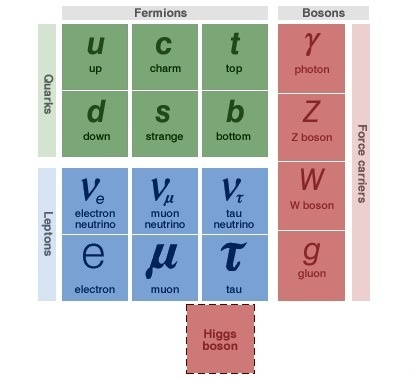
\includegraphics[width=\textwidth]{figures/figures/stdmod.jpg}
  \end{figure}
\end{columns}

}

\frame
{
  \frametitle{Neutrino Hypothesis  and Discovery}

  \begin{columns}[c]
  \column{0.5\textwidth}
  \centering
  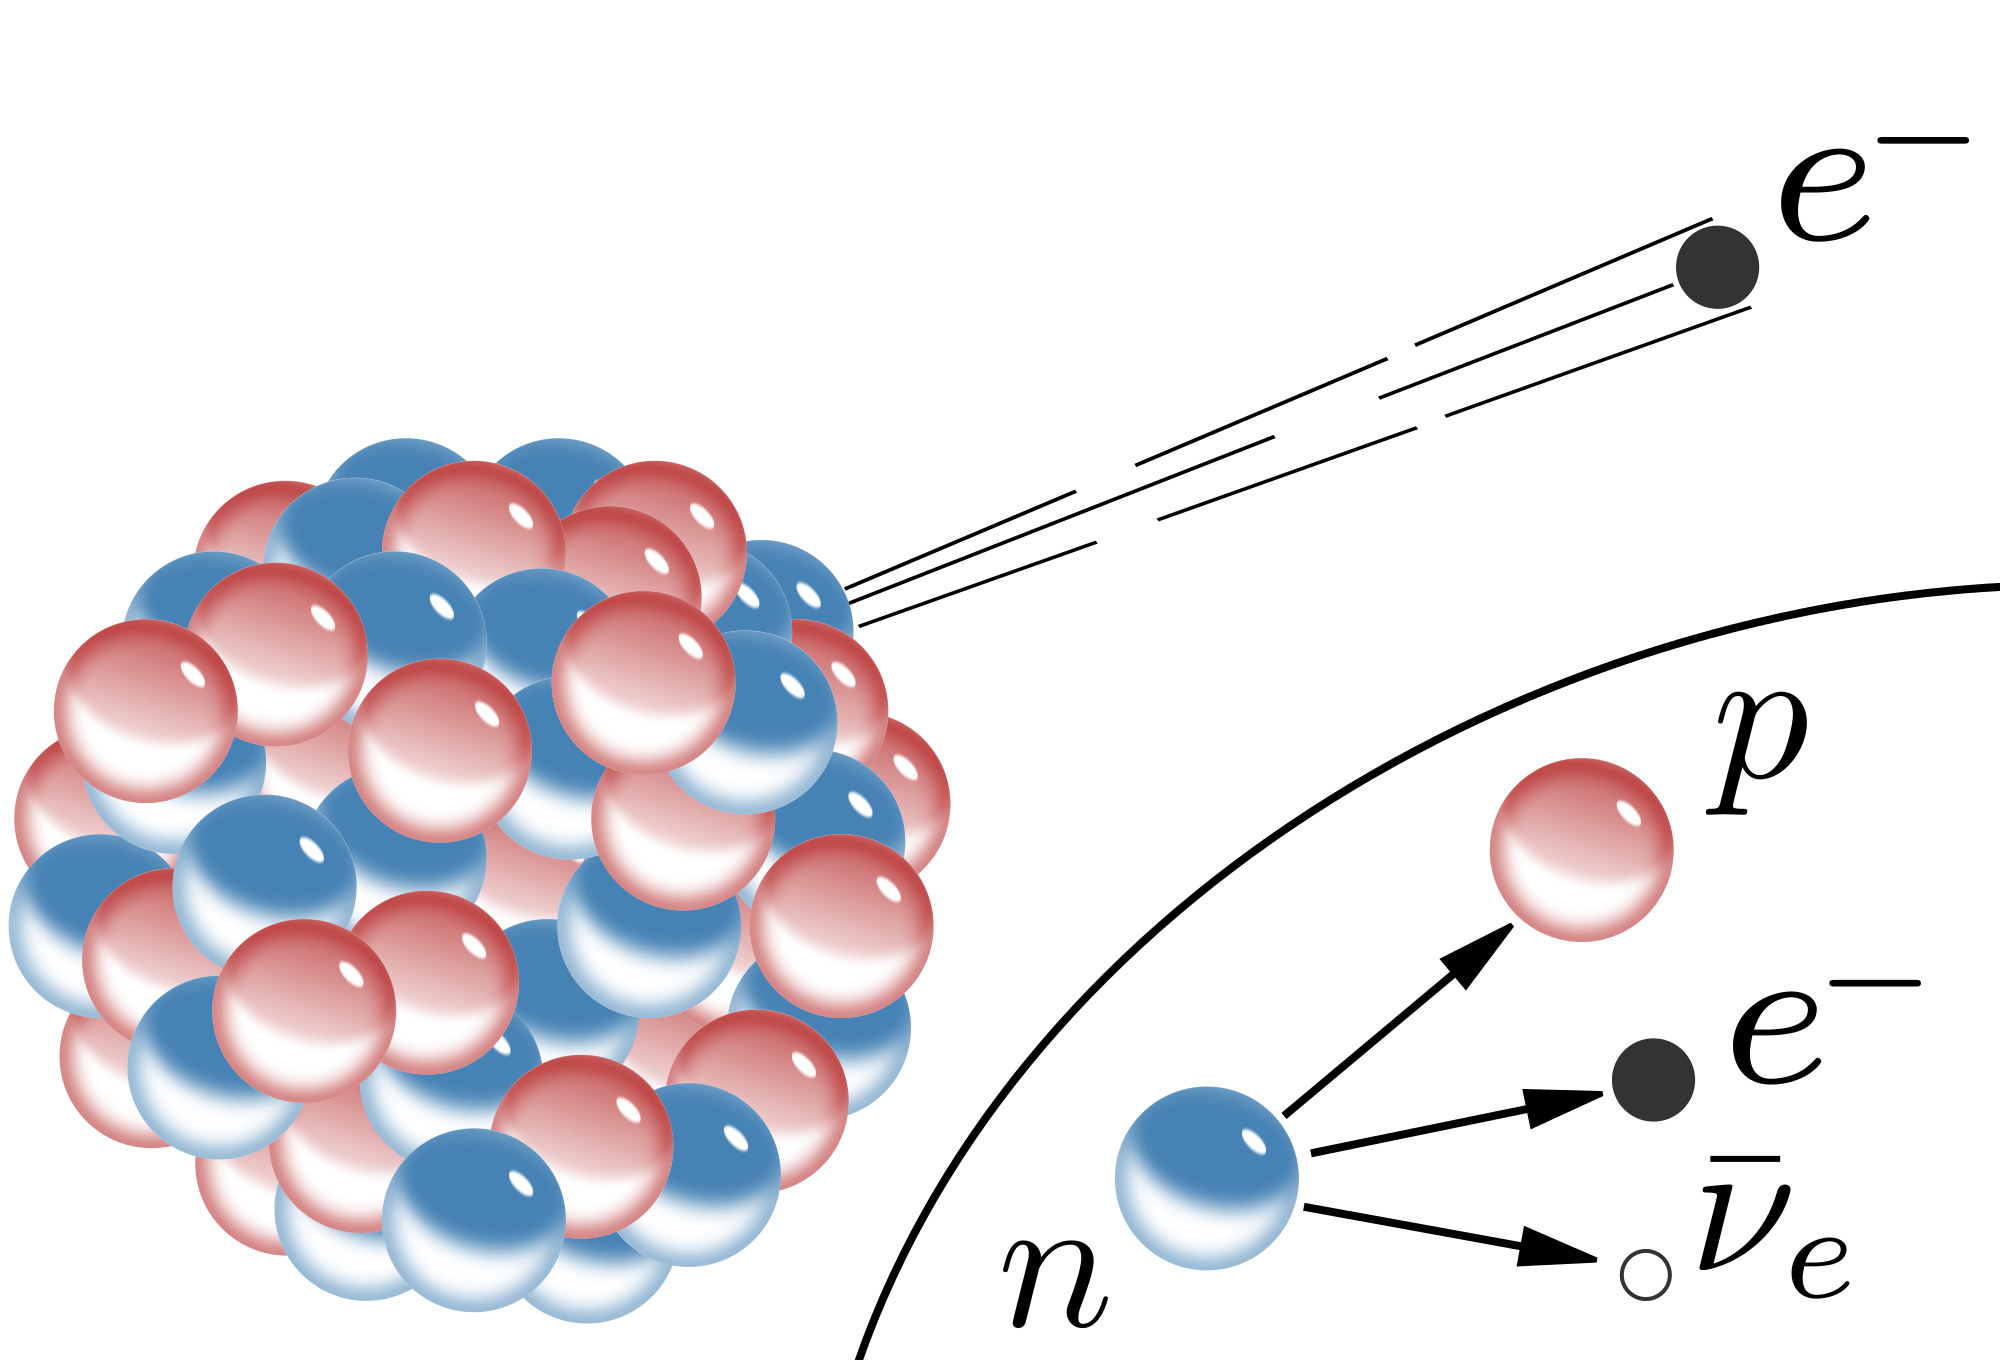
\includegraphics[height=0.37\textheight]{figures/figures/betaPretty.png}
  \column{0.5\textwidth}
  \centering
  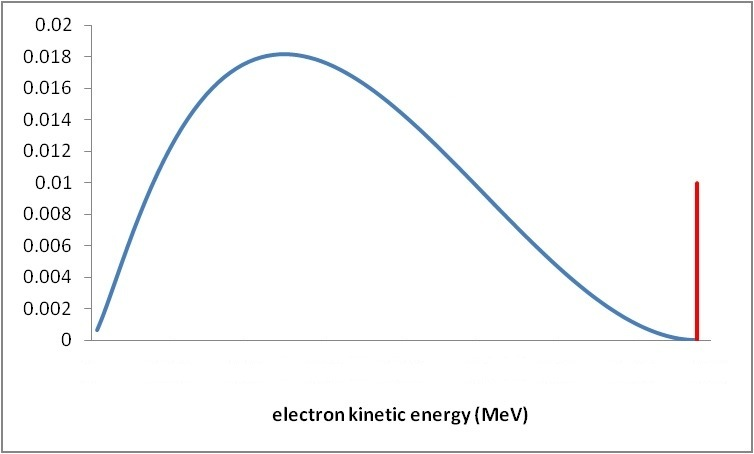
\includegraphics[height=0.37\textheight]{figures/figures/betaspec.jpg}
  \end{columns}
  \gap
  \begin{itemize}
  \bang Beta decay originally ($\sim$1900) seen as two body decay: $p \rightarrow n + e^-$
  \bang Conservation of momentum predicts single-valued energy spectrum for $e^-$
  \bang The spectrum they measured was in fact continuous
  \vspace{10pt}
  \bang Wolfgang Pauli postulated an unseen third particle
  \bang Enrico Fermi dubbed it neutrino, or ``little neutral one"
  \bang Neutrinos from nuclear reactors were experimentally observed in 1956
  \end{itemize}
}


\begin{frame}
  \frametitle{Neutrino Interactions}

  \bangon
  \bang Neutrinos are very small
    \bangon
    \bing ... i.e. they rarely interact with ordinary matter
    \bing Neutral to both electromagnetic and strong forces
    \bing Billions of them are passing through you right now without interacting
    \bing Could travel through a light-year of lead and probably not interact
    \bangoff
    \bangoff
    \gap
    \begin{columns}
      \column{0.5\textwidth}
  \centering
  \textcolor{custom_red}{Charged Current}


  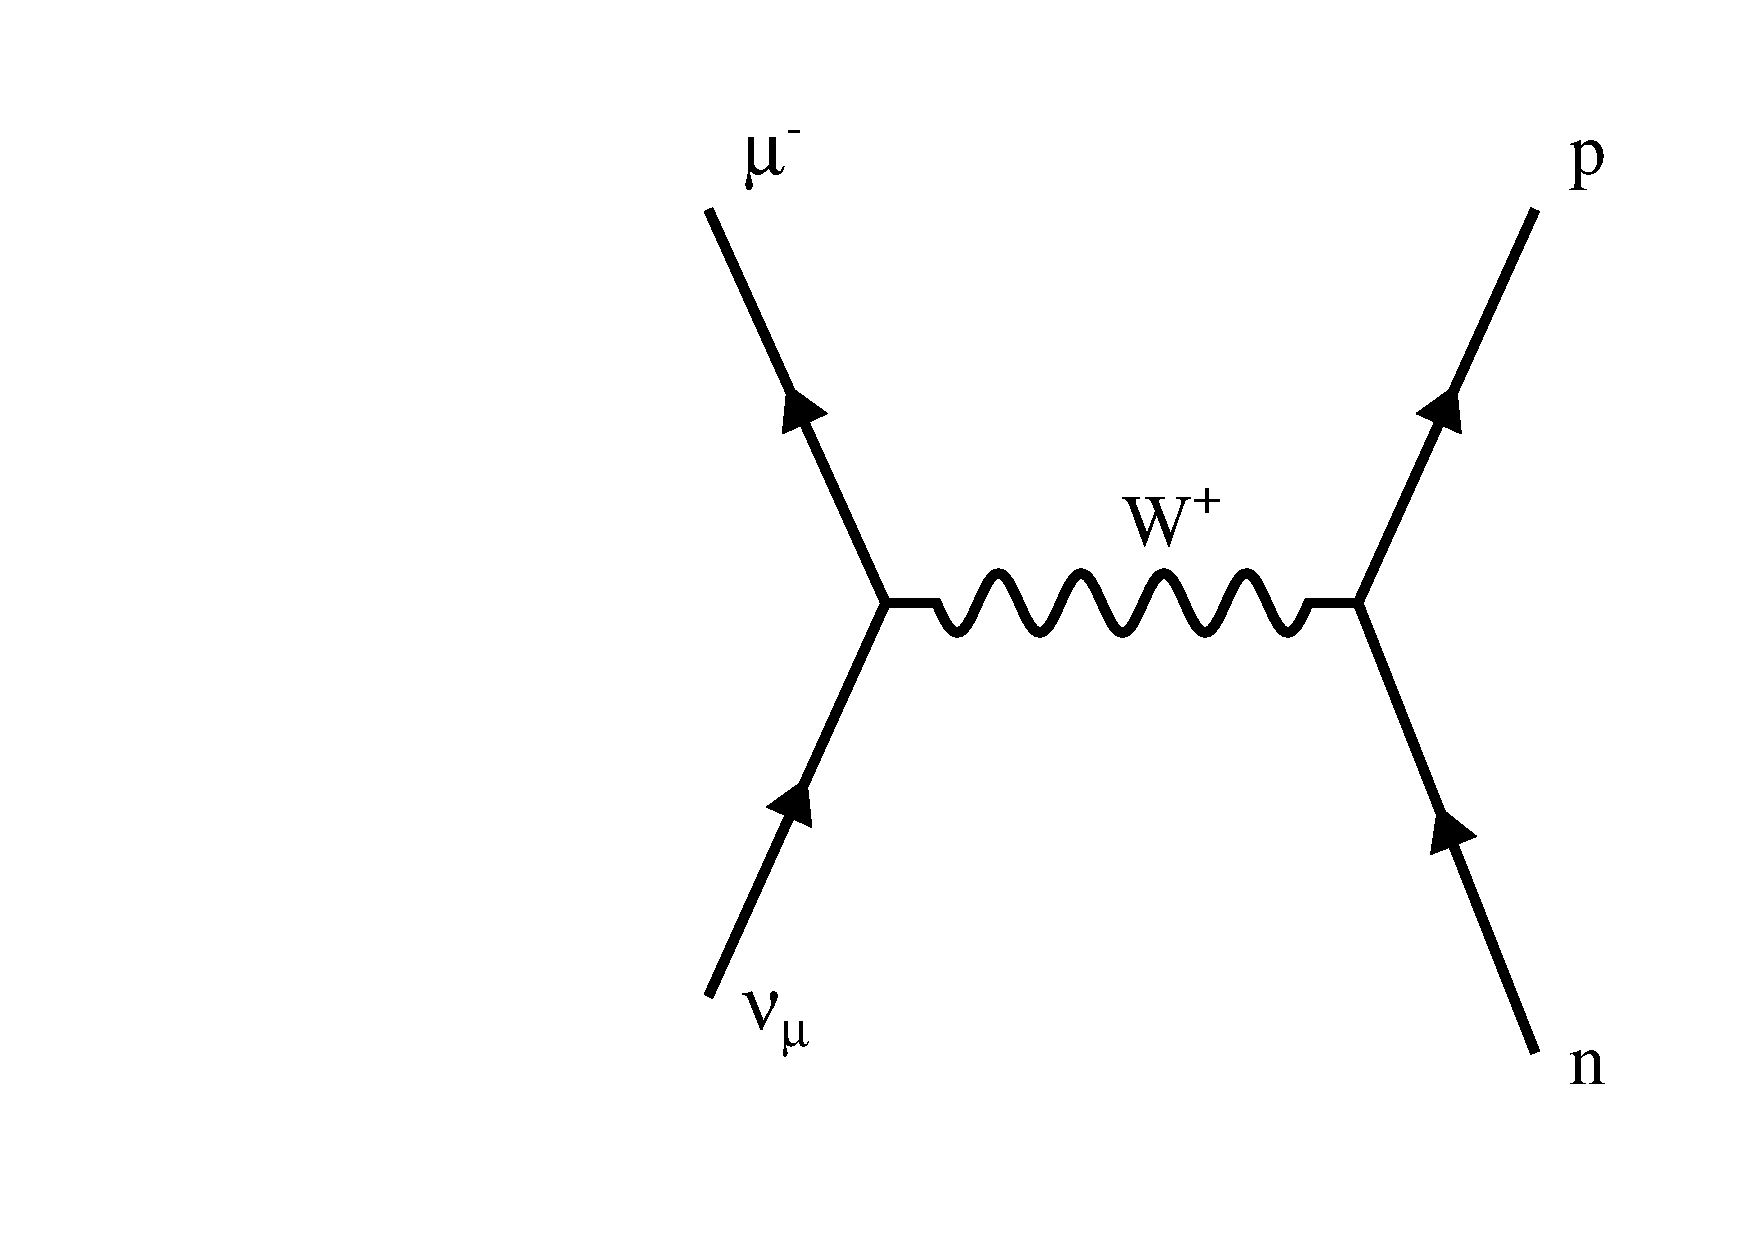
\includegraphics[height=0.37\textheight, angle=-90]{figures/feynman/ccNumu.pdf}
  \column{0.5\textwidth}
  \centering
   \textcolor{custom_red}{Neutral Current}


  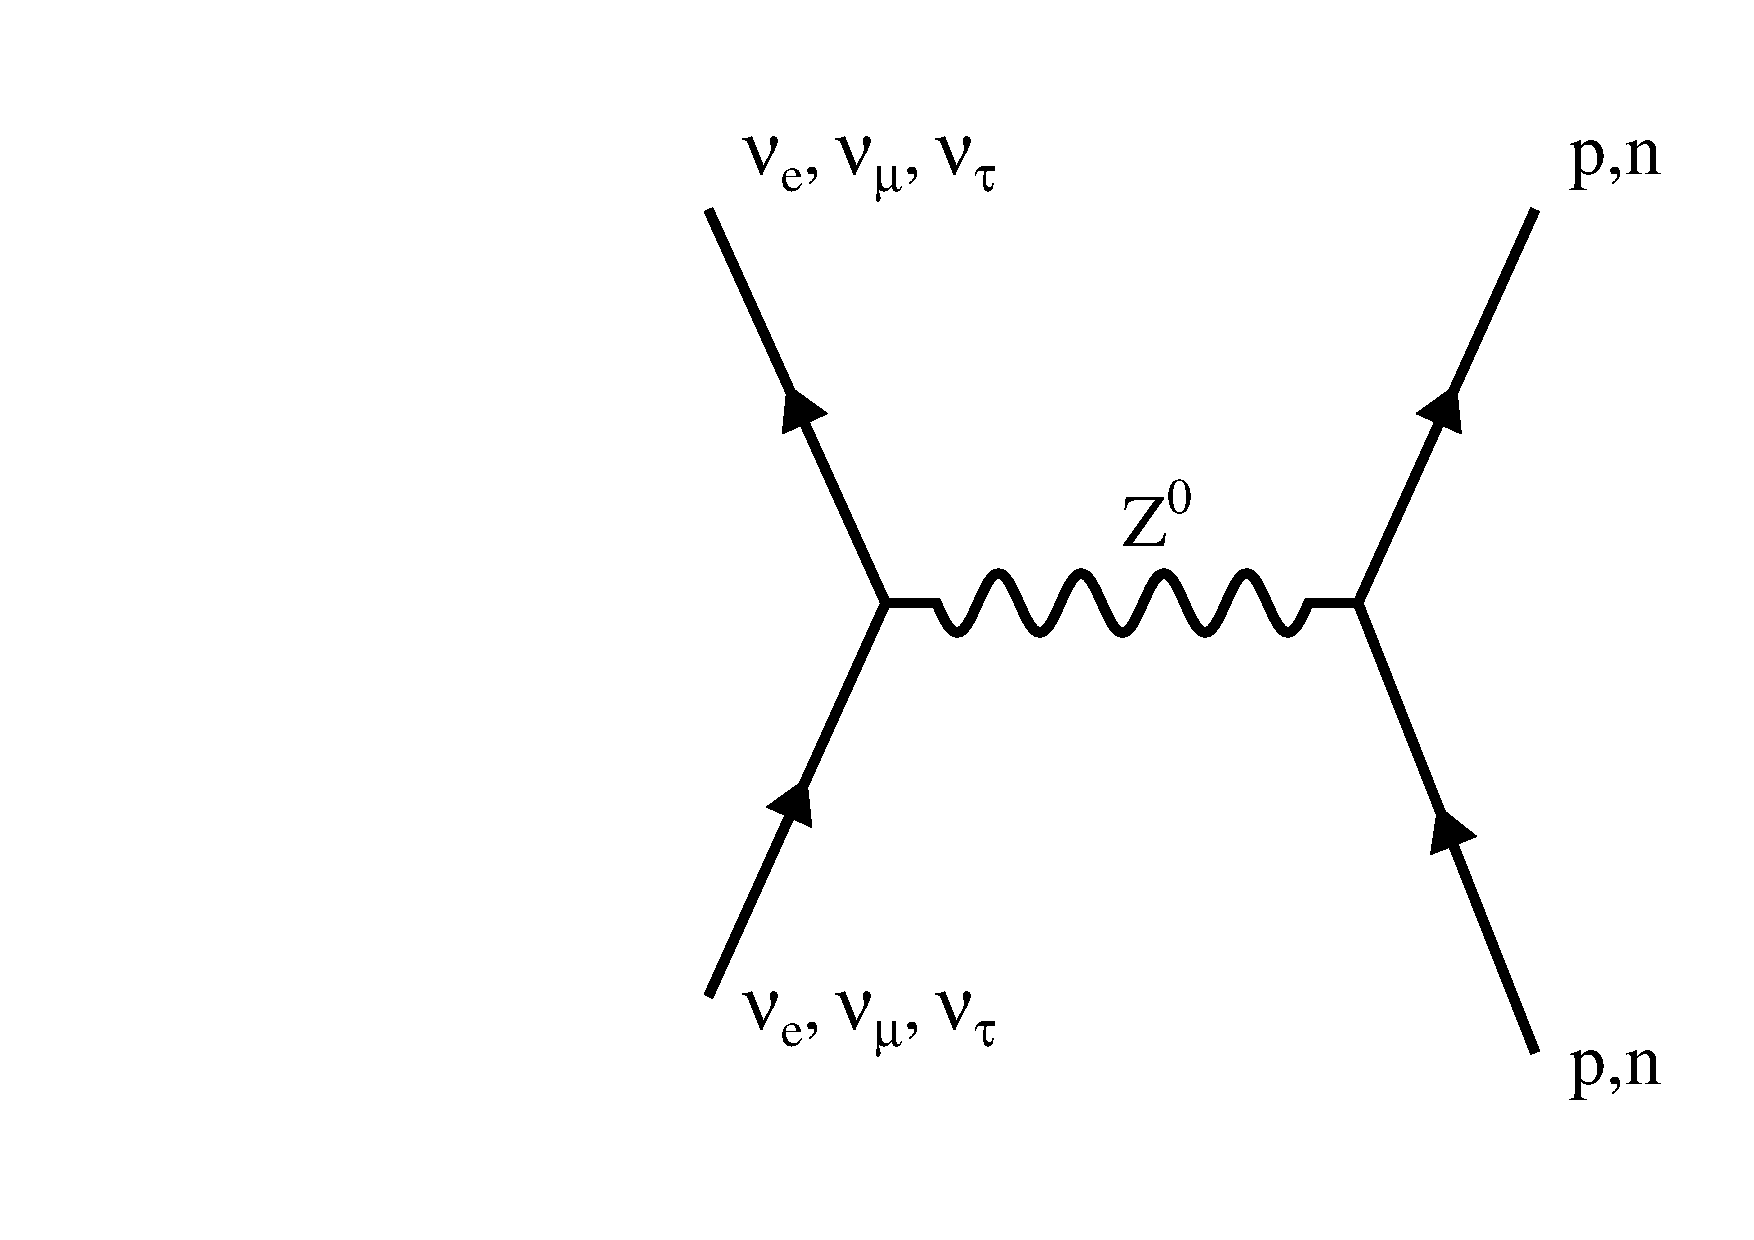
\includegraphics[height=0.37\textheight, angle=-90]{figures/feynman/ncHad.pdf}
  \end{columns}
\gap
    \bangon
    \item Weak interactions involve either $W$ or $Z$ bozon
      \bangon
      \item $W$: charged current
      \bong ~~~~ $\nu_e \rightarrow e$ ~~ or ~~ $\nu_\mu \rightarrow \mu$ ~~ or ~~ $\nu_\tau \rightarrow \tau$
      \item $Z$: neutral current
      \bong ~~~~ $\nu_e \rightarrow \nu_e$ ~~ or ~~ $\nu_\mu \rightarrow \nu_\mu$ ~~ or ~~ $\nu_\tau \rightarrow \nu_\tau$
      \bangoff
    \bangoff

\end{frame}

\frame
{
  \frametitle{Neutrino Oscillation}
  \bangon
  \bang Neutrinos change form as they travel
	  \bangon
	  \bing ... a.k.a. neutrino oscillation
	  \bing What starts as a $\nu_\mu$ could later be observed as an $\nu_e$ or $\nu_\tau$
	  \bing Probabilities of each changes based on distance travelled and neutrino energy
	  \bangoff
  \bangoff
\gap
\begin{columns}[c]
\column{0.45\textwidth}
\begin{equation*}
P_{\nu_\mu \rightarrow \nu_\mu} = 1 - \sin^2(2\theta) \sin^2\bigg(\frac{\Delta m^2 L}{4 E}\bigg)
\end{equation*}
\gap
\column{0.05\textwidth}
\vspace{-70pt}

\begin{equation*}
\color{blue}
\nu_\mu
\end{equation*}
\vspace{-20pt}
\begin{equation*}
\color{red}
\nu_\tau
\end{equation*}
\vspace{-20pt}
\begin{equation*}
\nu_e
\end{equation*}
\gap

\column{0.5\textwidth}
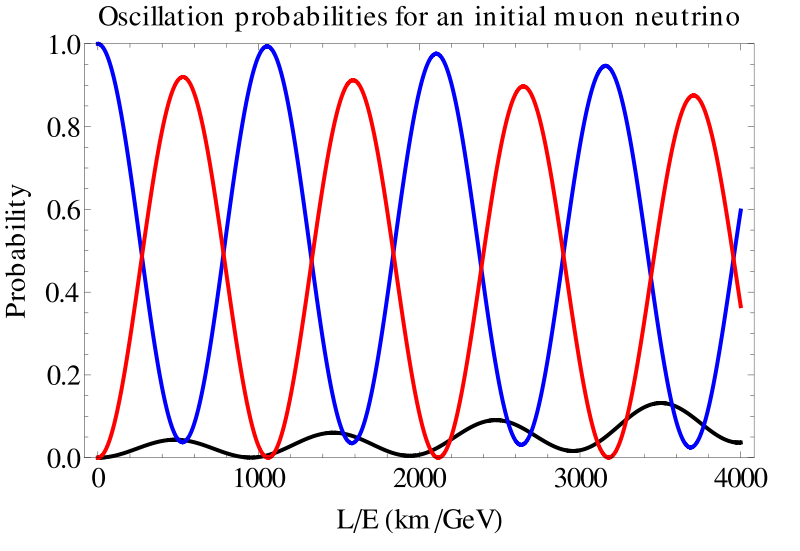
\includegraphics[width=1\textwidth]{figures/figures/osc_prob.png}

\end{columns}


}




\section{Neutrino Oscillations}
\frame
{
  \frametitle{Neutrino Oscillations in Vacuum}
  \begin{itemize}
  \bang Neutrinos are neutral leptons that interact weakly, they are produced in one of the flavor states.
  \bang In fact, each flavor state, $l=e,\mu,\tau$,  is a superposition of three distinct mass states, $\nu_1$, $\nu_2$, $\nu_3$:
  \begin{equation*}
|\nu_l(0) \rangle = \sum_{\alpha = 1,}^3 U_{l\alpha}|\nu_\alpha(0) \rangle.
  \end{equation*}
  \bang $U_{l\alpha}$ is an element in the Pontecorvo-Maki-Nakagawa-Sakata (PMNS) matrix\footnote{$c_{ij}$ and $s_{ij}$ denote $\cos(\theta_{ij})$ and $\sin(\theta_{ij})$, respectively. \vspace{3pt}}: 
  \begin{equation*}
 U = \begin{pmatrix} \label{pmns} 
c_{13}c_{12}              &    c_{13}s_{12} 	   	 & 		s_{13} e^{-i\delta} \\
-s_{12}c_{23} - c_{12}s_{23}s_{13}e^{i\delta}	& c_{12}c_{23} - s_{12}s_{23}s_{13}e^{i\delta} 				& 		c_{13}s_{23}  \\
s_{23}s_{12} - c_{12}c_{23}s_{13}e^{i\delta}	& -c_{12}s_{23} - s_{12}c_{23}s_{13}e^{i\delta} 				& 		c_{13}c_{23}  \\
\end{pmatrix}_{.}
\end{equation*}
\bang $U$ is a unitary matrix representing a rotation in a complex 3 dimensional space.
\bang $U$ depends on three Euler angles, $\theta_{12}$, $\theta_{23}$, $\theta_{13}$ and a phase $\delta$ representing CP violation.
  \end{itemize}
}

\frame
{
  \frametitle{Neutrino Oscillations in Vacuum}
  \begin{itemize}
	\bang Oscillations are given by time evolution:
	\begin{equation*}
		|\nu_l(t) \rangle = \sum_{\alpha = 1,}^3 U_{l\alpha}e^{-iE_\alpha t}|\nu_\alpha(0) \rangle
	\end{equation*}
	\bang For relativistic neutrinos, we approximate the energy and take $t \rightarrow L$, which we substitute into the time evolution:
	\begin{equation*}
		|\nu_l(L) \rangle = e^{-iEL} \sum_{\alpha = 1,}^3 U_{l\alpha}e^{-i\frac{m_\alpha^2}{2E} L}|\nu_\alpha(0) \rangle.
	\end{equation*}
	\bang The factor $e^{-i\frac{m_\alpha^2}{2E} L}$ gives rise to oscillations. 
	\bang We then find the oscillation probability:
	\begin{equation*}\begin{split}
P_{l\rightarrow m}(L) =  \delta_{lm} - 4  \sum_{\alpha > \beta}  \Re(U^*_{l\alpha}U_{m\alpha}U^*_{l\beta}U_{m\beta}) \sin^2 \bigg(\frac{\Delta m_{\alpha\beta}^2}{4E} L\bigg) \\
 + 2  \sum_{\alpha>\beta}  \Im(U^*_{l\alpha}U_{m\alpha}U^*_{l\beta}U_{m\beta}) \sin\bigg(\frac{\Delta m_{\alpha\beta}^2}{2E}L\bigg).
\end{split}\end{equation*}
	\bang All time dependence is wrapped up in the $\sin$ terms, the prefactors are real constants that depend on the mixing angles.  


  \end{itemize}
}

\section{Oscillation Parameter Measurements}
\frame
{
  \frametitle{Current Oscillation Parameter Measurements}
    \begin{itemize}
   \bang Solar neutrino experiments have measured $\sin^2(2 \theta_{12}) $ and $\Delta m_{21}^2$ .
   \bang Long-baseline and atmospheric  neutrino experiments have measured $\sin^2(2 \theta_{23}) $ and $|\Delta m_{32}^2|$ .  
   \bang $\sin^2(2 \theta_{13})$ has recently been measured to be nonzero.  
\bang The CP-violating phase $\delta$ has never been measured.
\bang The ordering of the mass hierarchy is unknown, that is, the sign of $\Delta m_{32}^2$.
\end{itemize}
\begin{columns}[c]
\column{0.5\textwidth} \footnotesize
\begin{tabular}{ |c |  c| }
\hline  
Parameter & PDG Average\footnote{J. Beringer et al. (Particle Data Group), Phys. Rev. D86, 010001 (2012)} \\  \hline  
  $\sin^2\big(2 \theta_{12}\big)$&$  0.875 \pm0.024$  \\ 
  $\sin^2\big(2 \theta_{23}\big)$&$  > 0.95                  $   \\ 
  $\sin^2\big(2 \theta_{13}\big)$&$  0.098 \pm0.013$  \\ 
    $\Delta m^2_{21}       $&$ (7.50 \pm 0.2) \times 10^{-5}$ eV${}^2$ \\
  $|\Delta m^2_{32}|       $&$ (2.32^{+0.12}_{-0.08} ) \times 10^{-3}$ eV${}^2$  \\
  \hline  
\end{tabular}
\column{0.5\textwidth}
 \begin{figure} 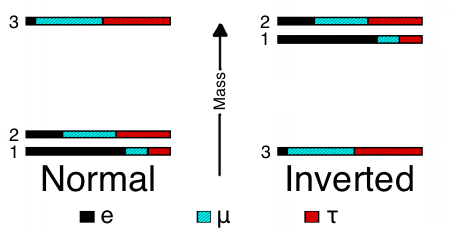
\includegraphics[width=\textwidth]{hierarchy.jpg} \end{figure}
 \vspace{8pt} 
\end{columns}

}





\frame
{
\frametitle{\nova}

\begin{columns}[c]
\column{0.6\textwidth}

\begin{itemize}
\bang  \textbf{NuMI} is a neutrino source at Fermilab
\bong (Neutrinos at the Main Injector)
  \bangon
  \bing Mostly \numu
  \bangoff
\gap
\bang \textbf{\nova} is a neutrino oscillation experiment
\bong (NuMI Off-axis $\nu_e$ Appearance)
  \bangon
  \bing Two functionally identical detectors
  \bing 14 mrad off-axis
  \bing Narrow energy peak near 2 GeV

  \bangoff
\gap

\end{itemize}
\centering \footnotesize
\gap
\begin{tabular}{l | c | c}
& Near Detector & Far Detector  \\ \hline
Baseline (km)& 1  & 810   \\ \hline
Mass (kton) & 0.3 & 14  \\ \hline
%Channels & 20,192 & 344,064  \\ %\hline
\end{tabular}

%{ \centering
%\includegraphics[width=1\textwidth]{figures/earth.png}}

\column{0.4\textwidth}
\centering
\vspace{-5pt}
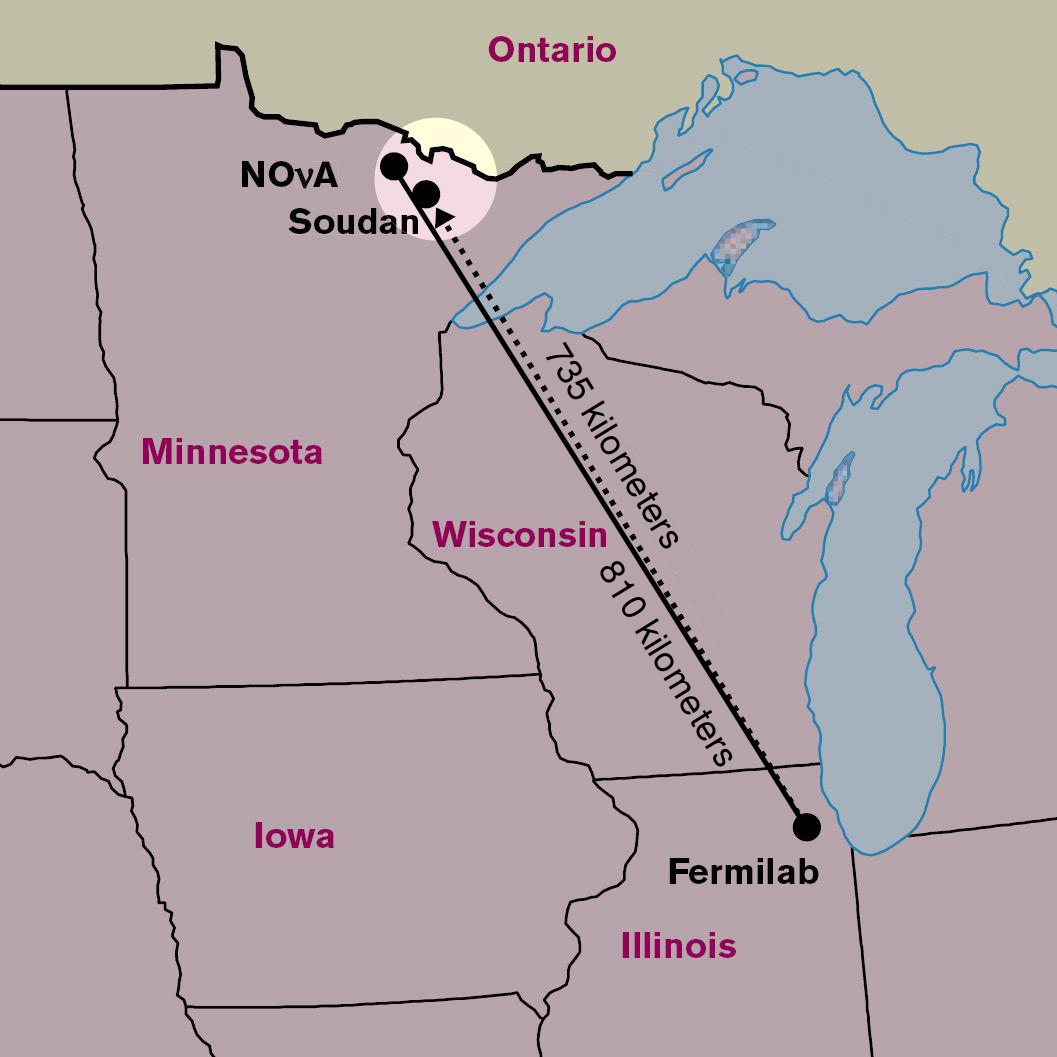
\includegraphics[width=1\textwidth]{figures/figures/map.png}

\vspace{7pt}

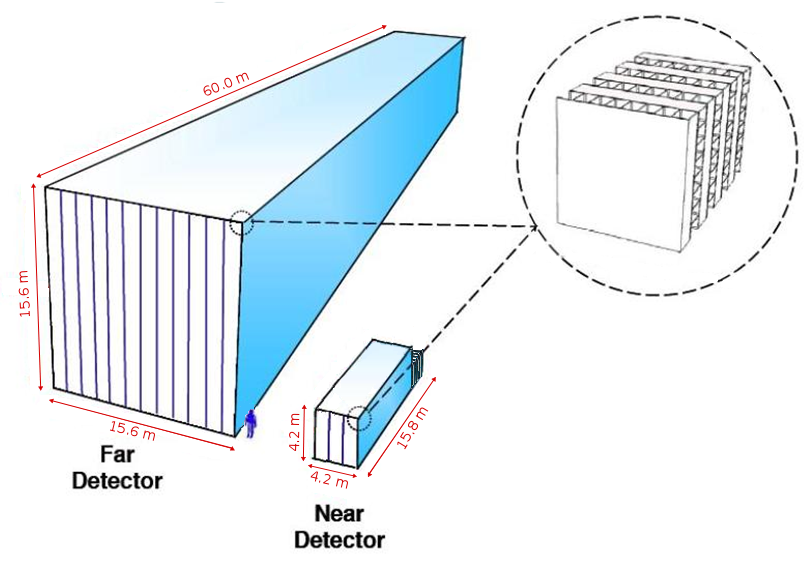
\includegraphics[width=1\textwidth]{figures/figures/detectors.png}

\end{columns}


}

\frame
{
  \frametitle{NuMI}
    \begin{itemize}
	\bang High energy protons from are directed into a graphite target
	\bang These collisions produce a shower of particles
	\bang Shower is primarily pions and kaons
	\bang Muons are absorbed in steel plates and rock to leave behind a beam of muon-neutrinos
	\begin{figure} 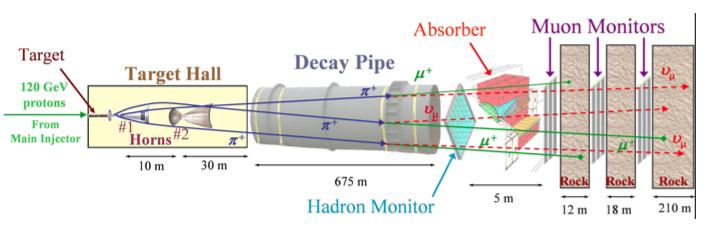
\includegraphics[width=0.85\textwidth]{figures/figures/numi.png} \end{figure}
\end{itemize}

}

\frame
{
\frametitle{\nova Detectors}

\bangon
\bang Basic unit of \nova detectors is an extruded PVC cell
\bang Cells are filled with liquid scintillator
\bang Wavelength-shifting fiber transmits scintillation light to readout
\bang Avalanche photo-diodes capture light output from fiber
\bangoff

\begin{columns}[c]
\column{0.15\textwidth}
 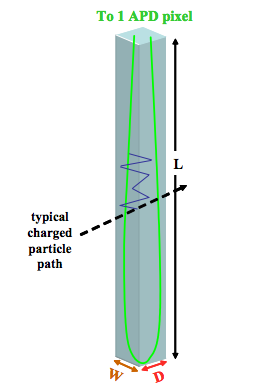
\includegraphics[width=1.4\textwidth]{figures/figures/cell.png}
\column{0.02\textwidth}
~
\column{0.83\textwidth}

\centering
 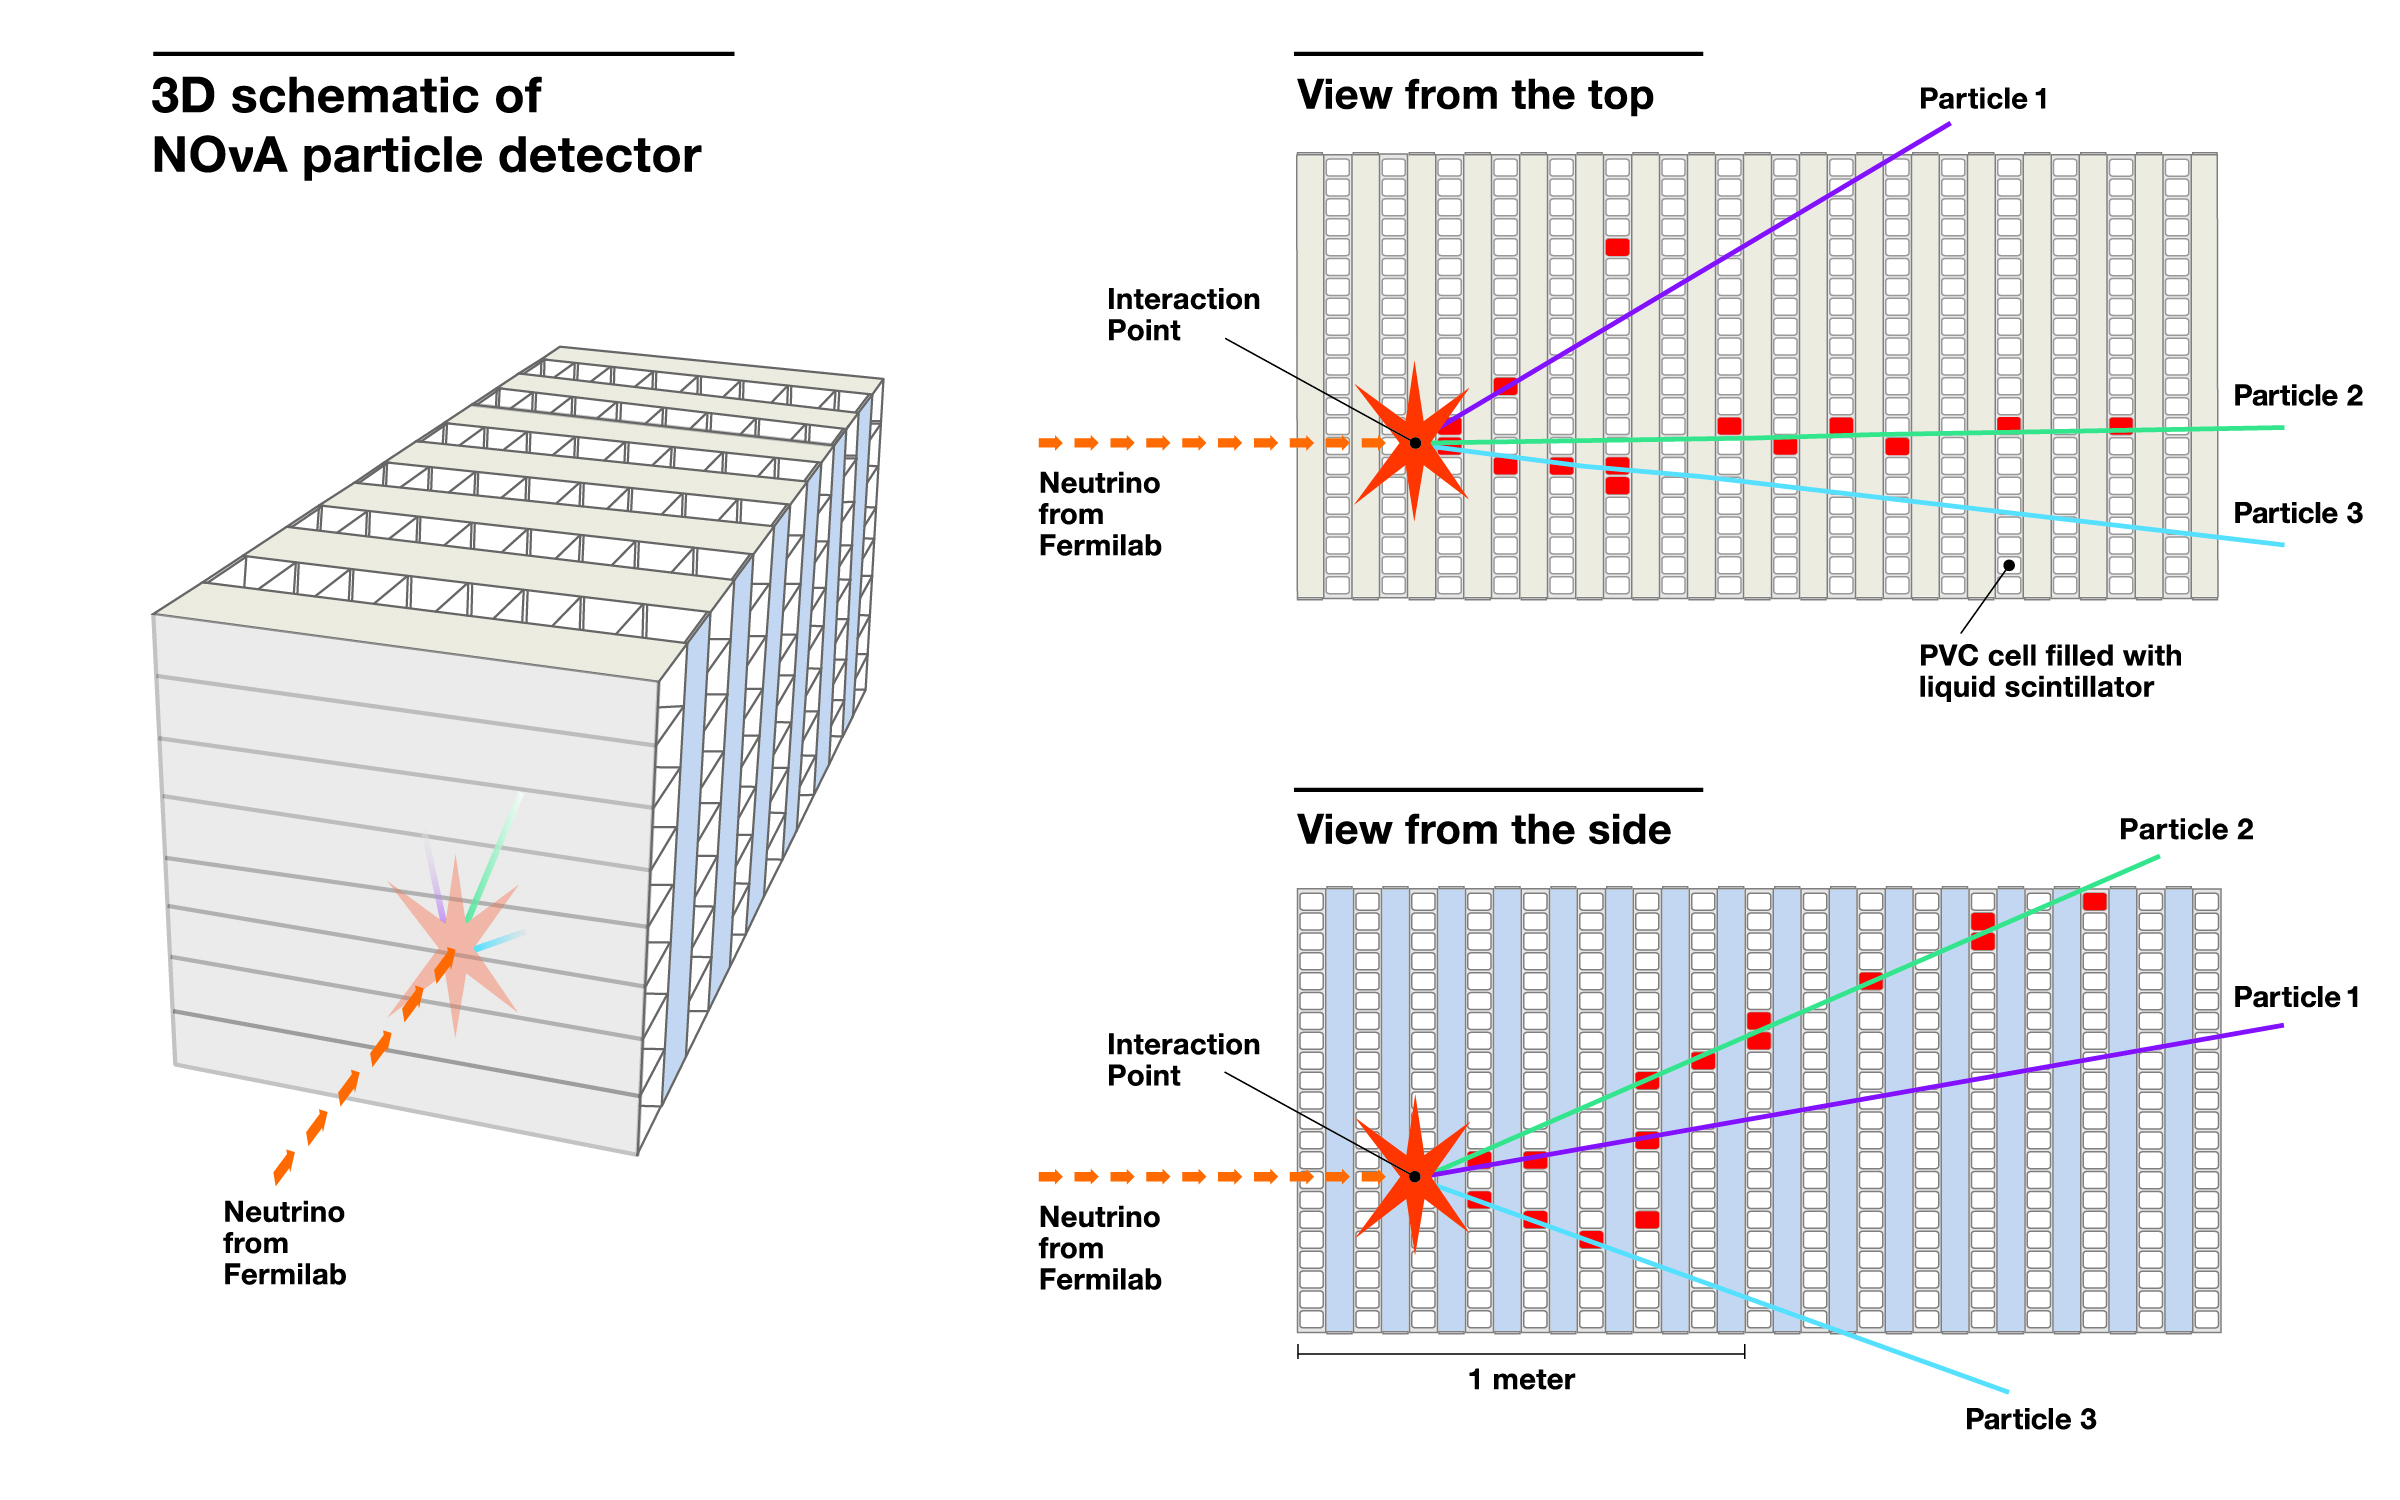
\includegraphics[width=0.85\textwidth]{figures/figures/schematic.jpg}

 {\scriptsize Illustration courtesy of Fermilab}

\end{columns}




}




\frame
{
  \frametitle{Far Detector}
  \centering
\begin{columns}[c]
\column{0.5\textwidth}
\centering
 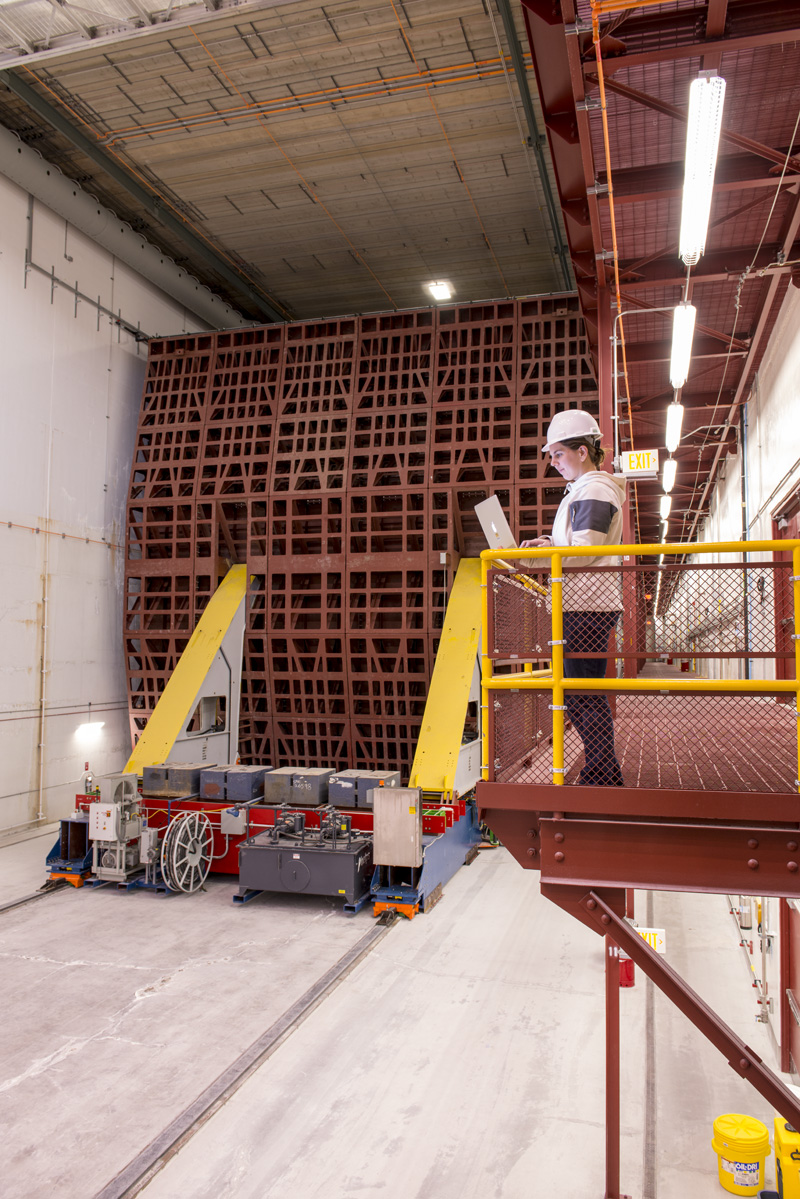
\includegraphics[height=0.85\textheight]{figures/det_photos/det_front.jpg}

\column{0.5\textwidth}
\centering
 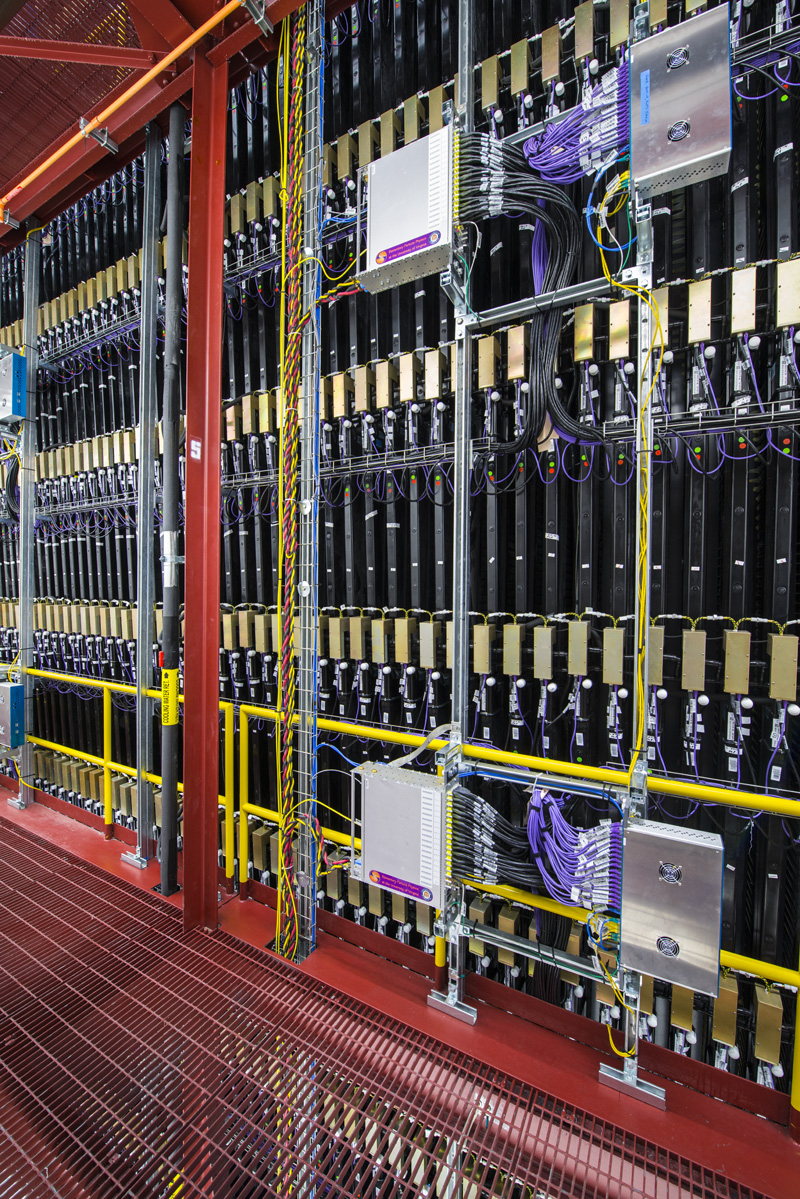
\includegraphics[height=0.85\textheight]{figures/det_photos/det_side.jpg}
\end{columns}
\gap
{\scriptsize Photos courtesy of Fermilab}


}

\frame
{
  \frametitle{Near Detector}
    \begin{itemize}
	\bang The Near Detector is considerably smaller
	\bang Installed in a 300 foot deep cavern at Fermilab

\end{itemize}
	\begin{figure} \includegraphics[height=0.55\textwidth]{figures/det_photos/ND.jpg} \end{figure}
}


\frame
{
  \frametitle{Near Detector}
	\begin{figure} 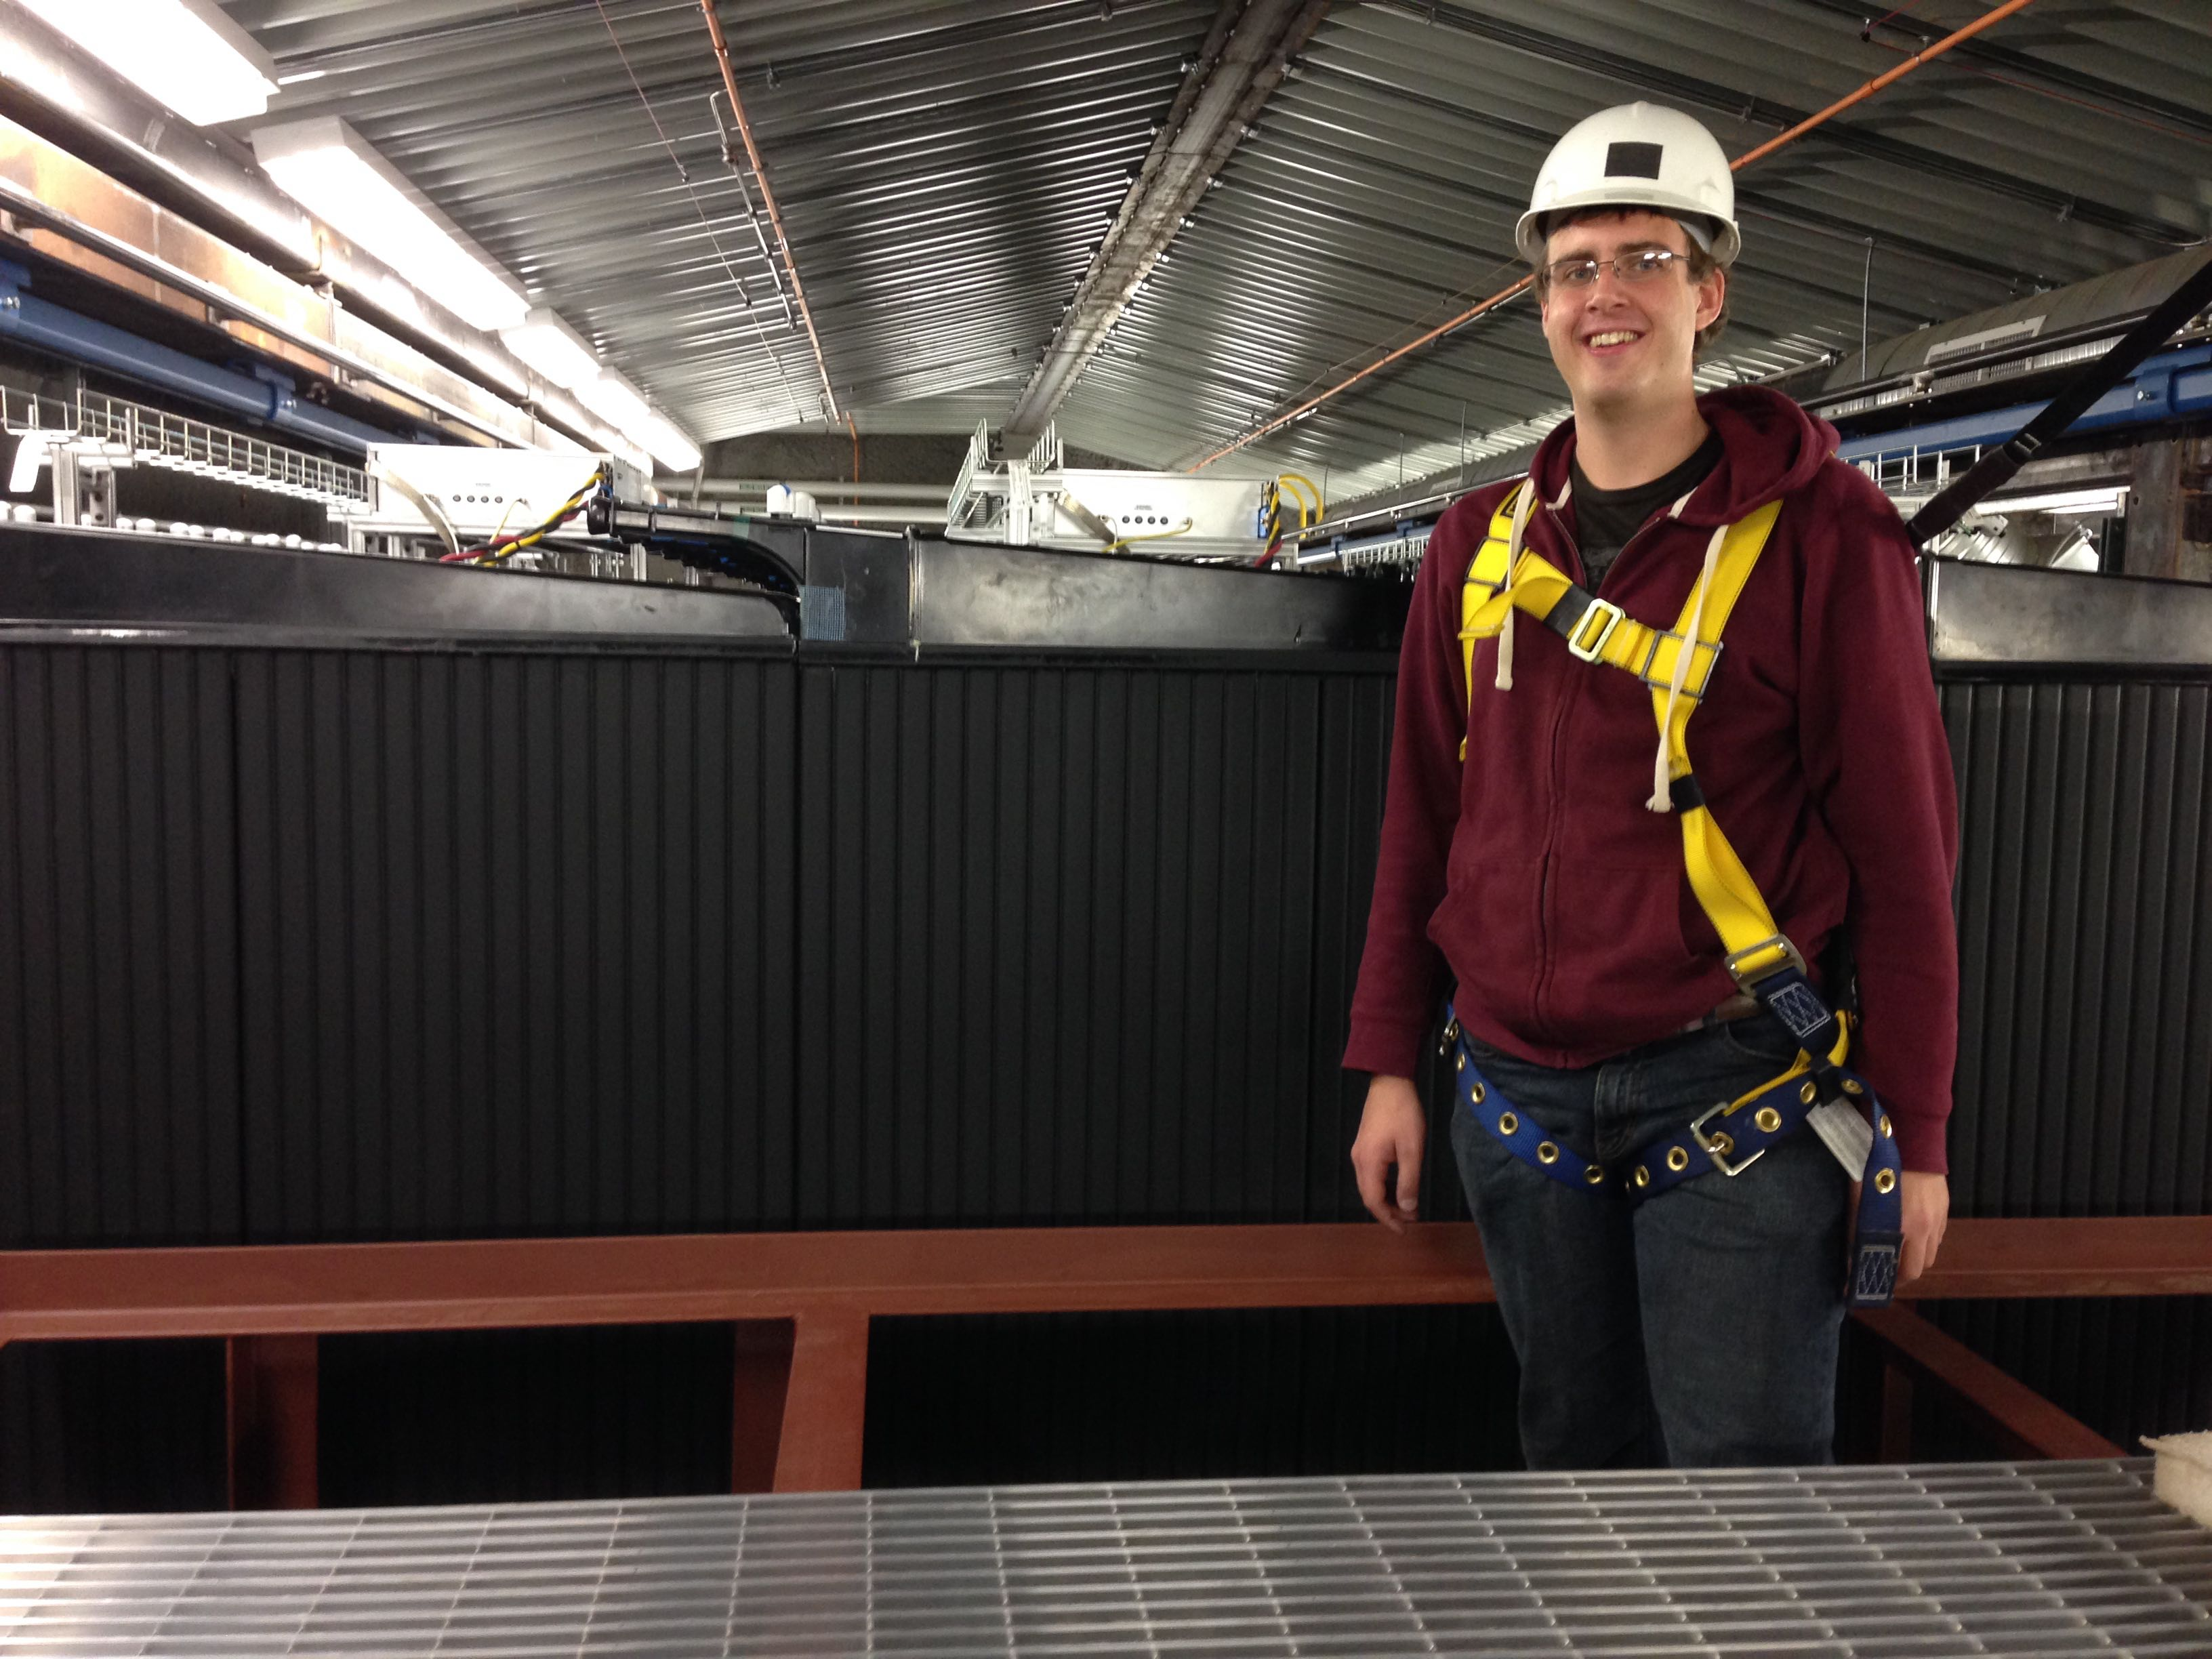
\includegraphics[height=0.55\textwidth]{figures/det_photos/meND_small.jpg} \end{figure}
}

\frame
{
  \frametitle{Event Topologies}

 \begin{figure} 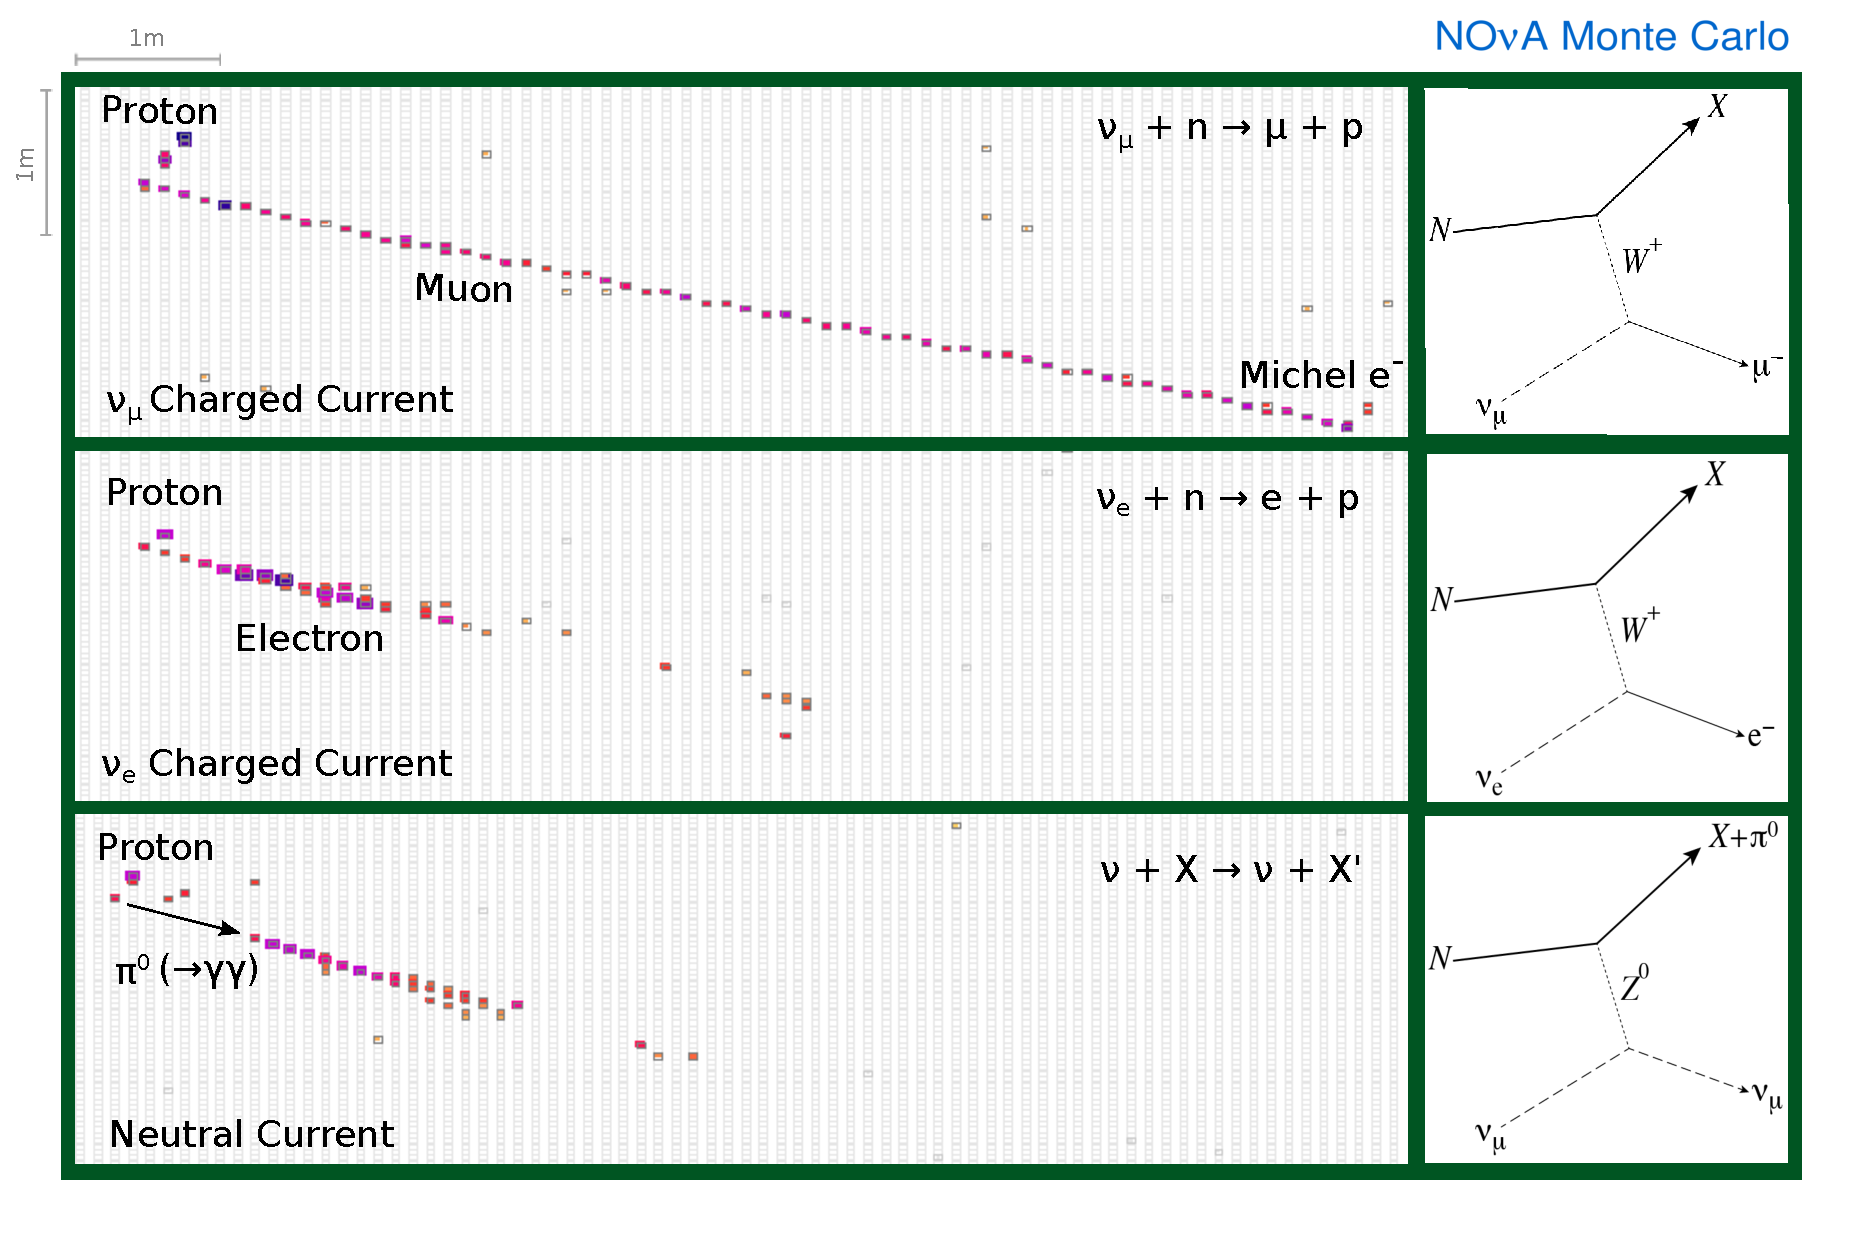
\includegraphics[width=0.95\textwidth]{figures/figures/event_topology_nue.pdf} \end{figure}
}


\frame
{
  \frametitle{Real Far Detector Data}

 \begin{figure} 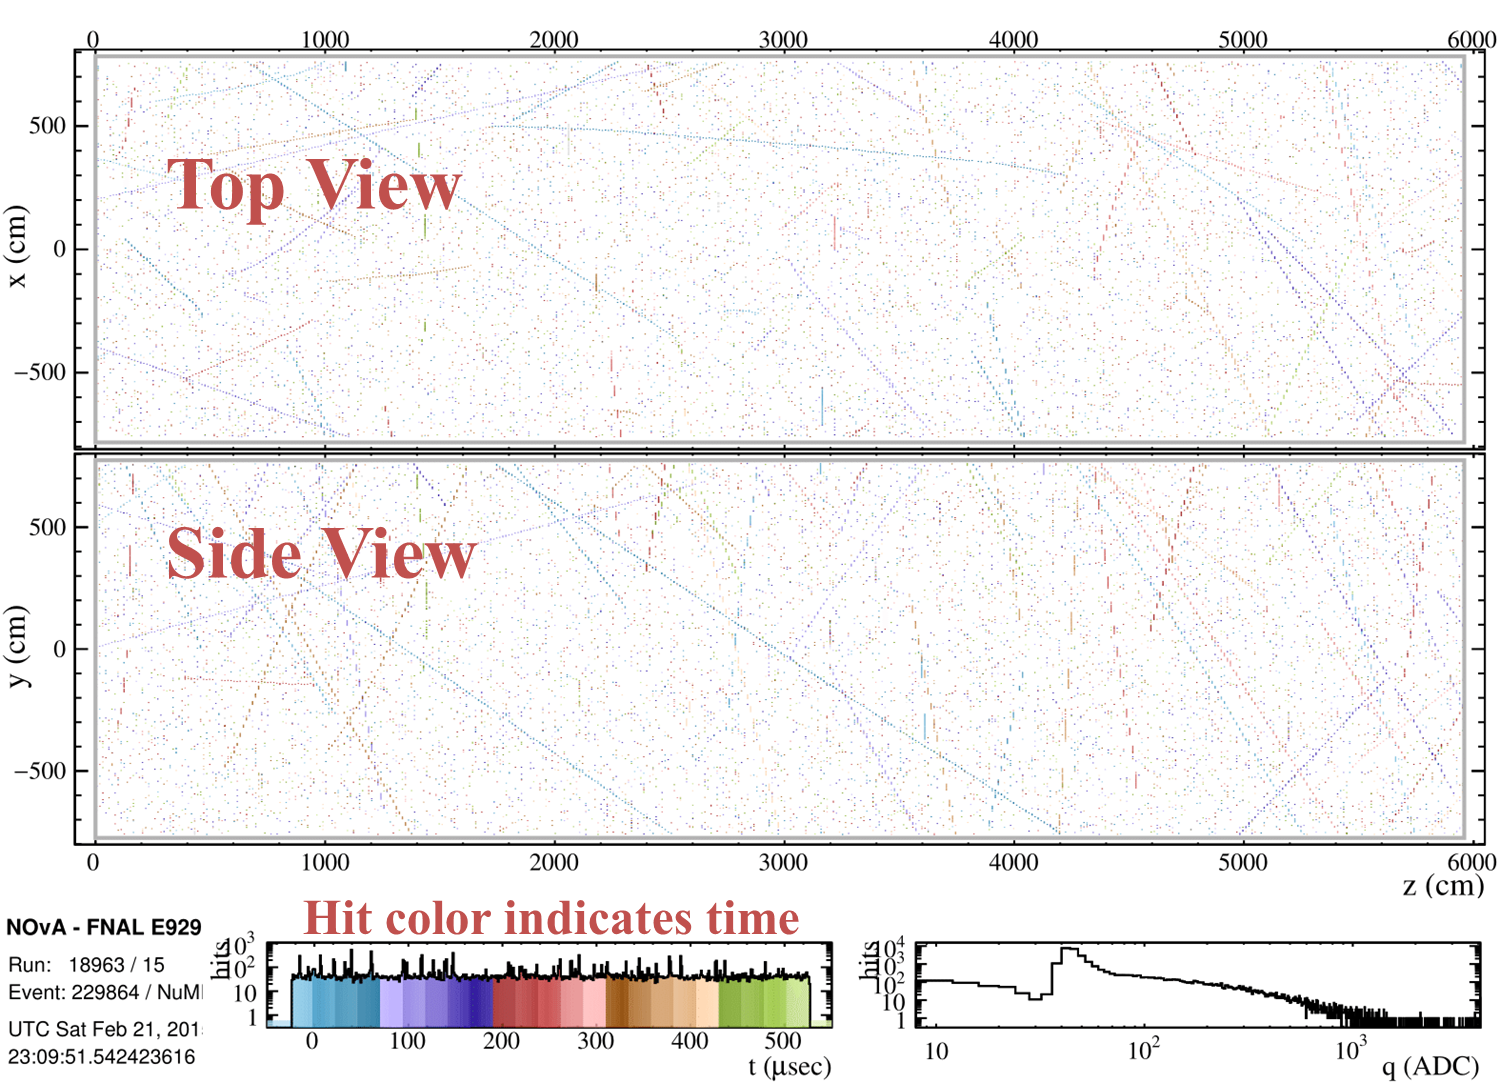
\includegraphics[width=0.9\textwidth]{figures/evd_steps/evd_top_side.png} \end{figure}
}

\frame
{
  \frametitle{Real Far Detector Data}

 \begin{figure} 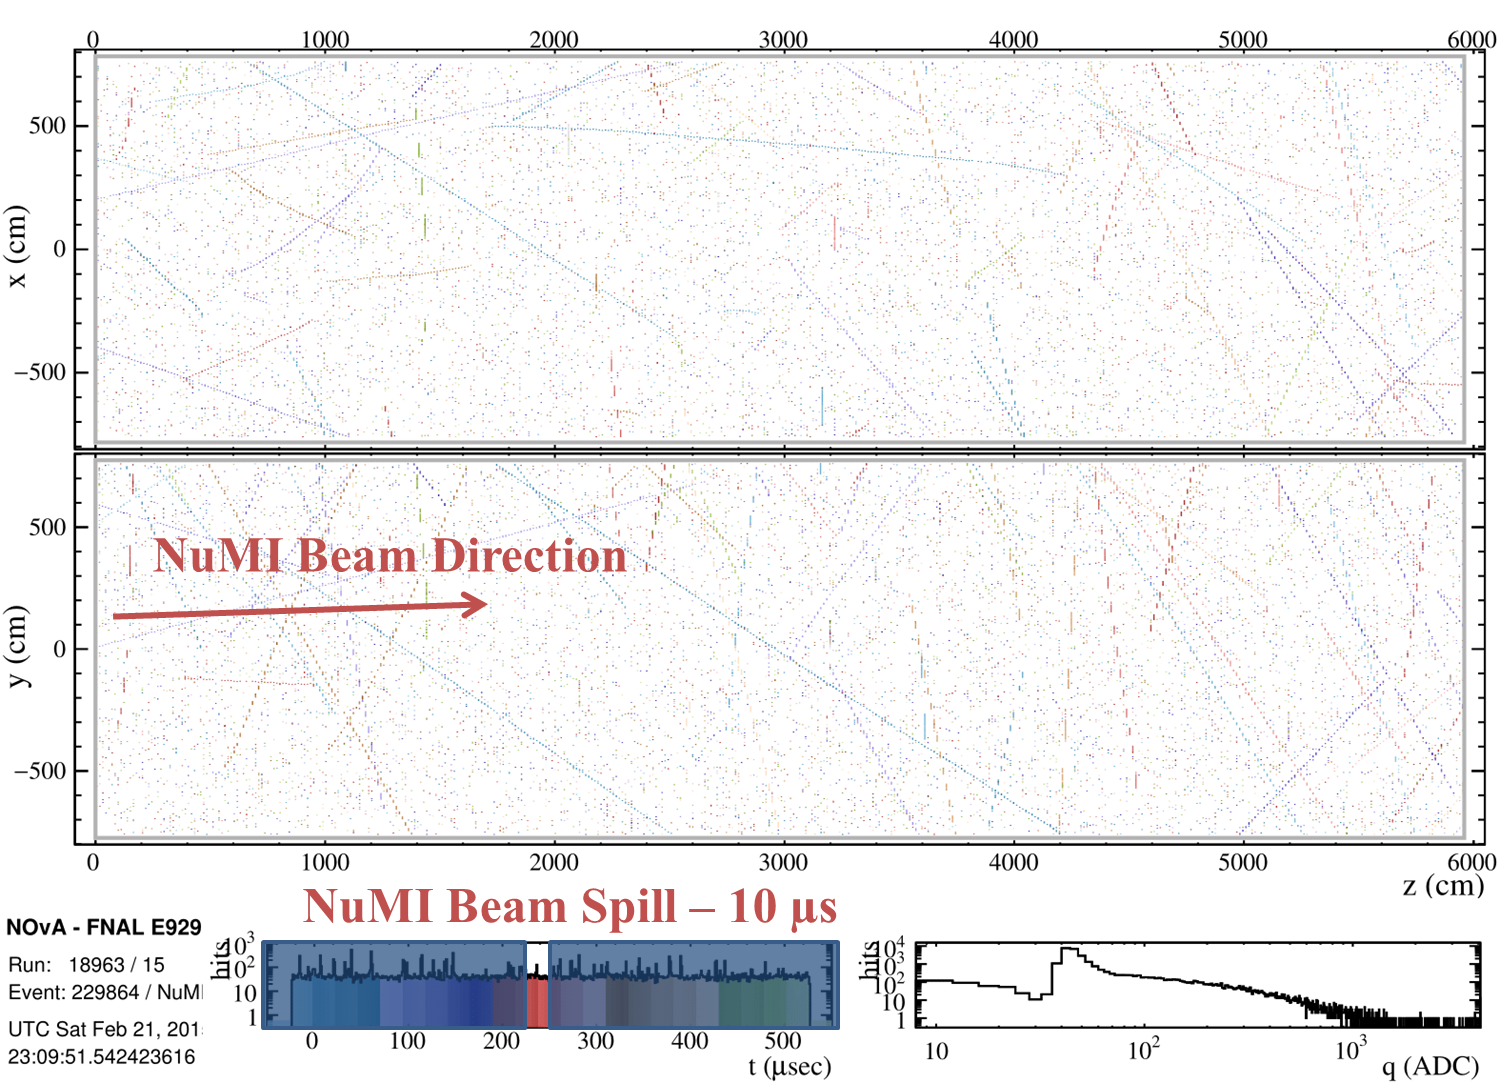
\includegraphics[width=0.9\textwidth]{figures/evd_steps/evd_beam_dir.png} \end{figure}
}

\frame
{
  \frametitle{Real Far Detector Data}

 \begin{figure} 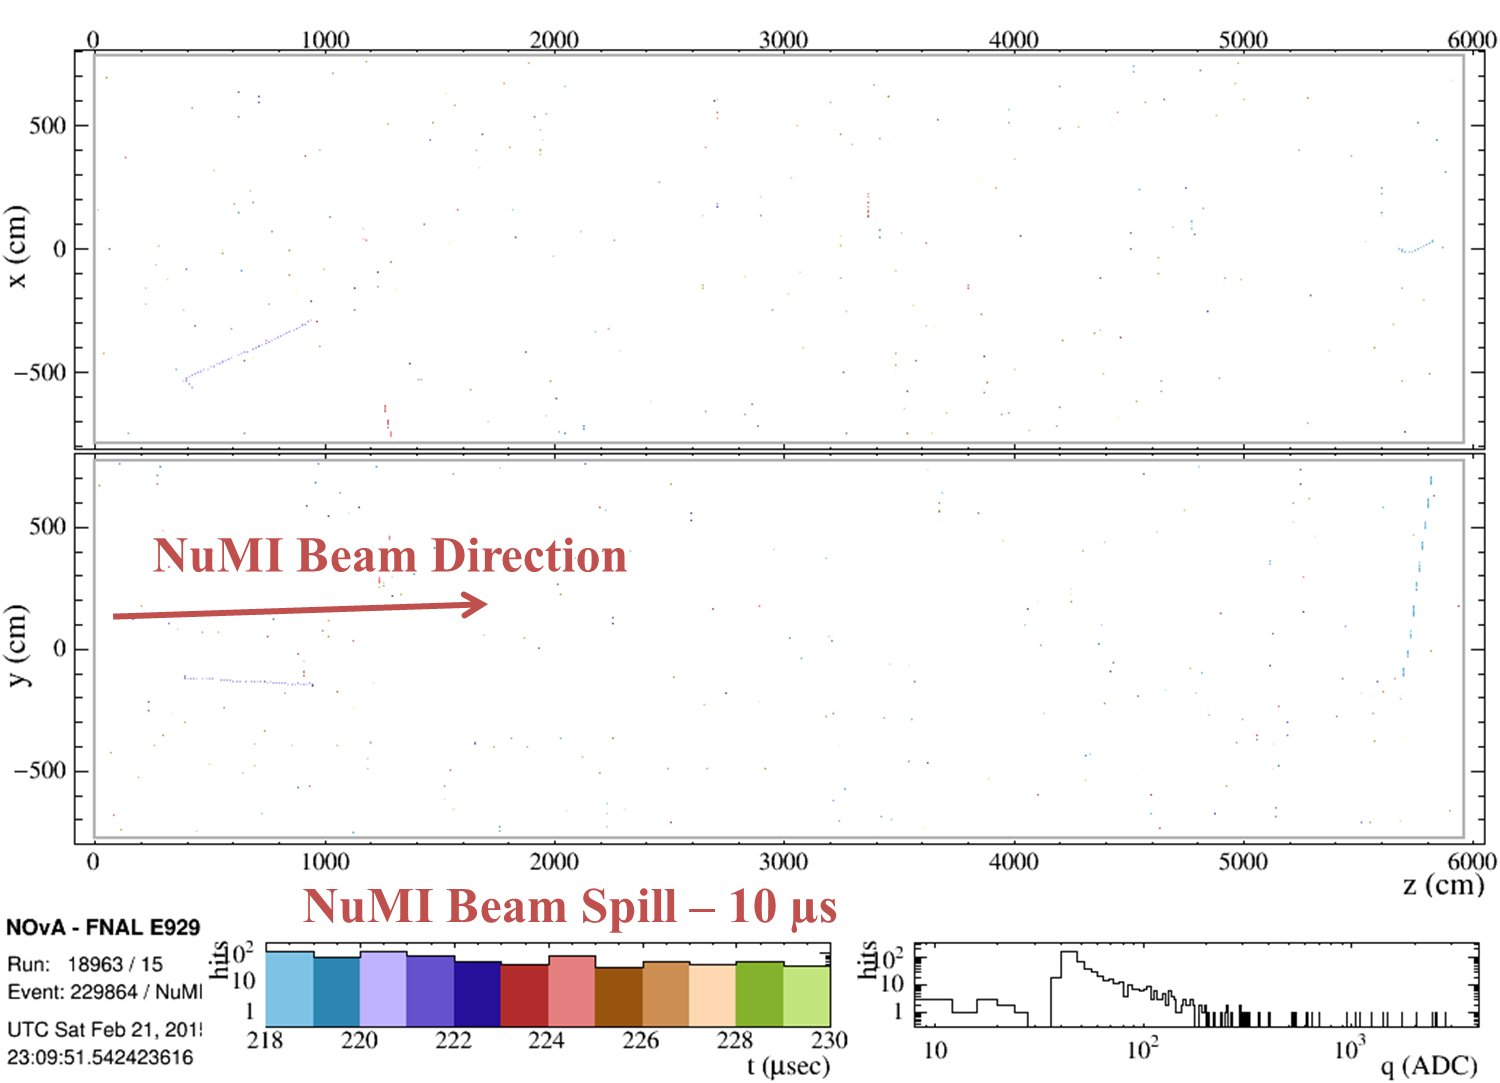
\includegraphics[width=0.9\textwidth]{figures/evd_steps/evd_beam_dir_nu.png} \end{figure}
}

\frame
{
  \frametitle{Real Far Detector Data}

 \begin{figure} 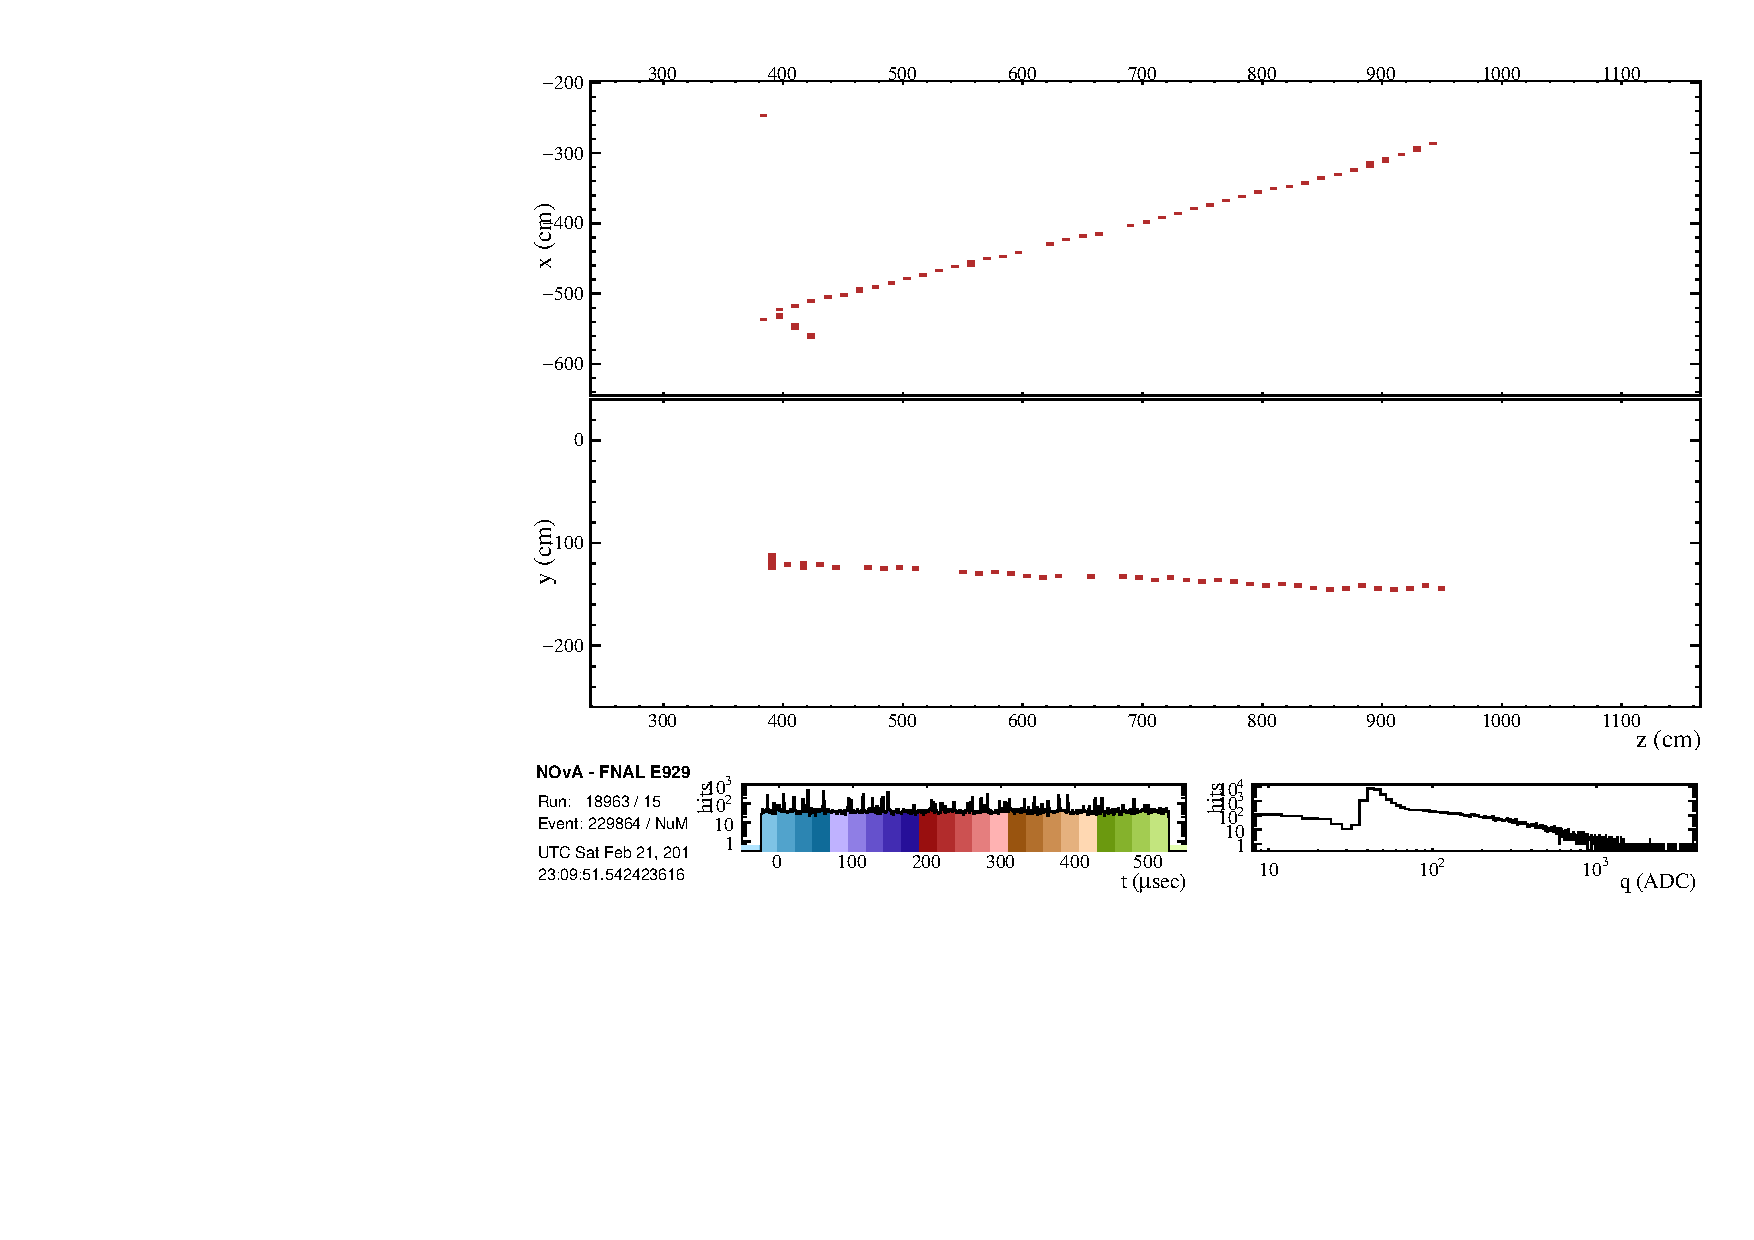
\includegraphics[height=0.9\textwidth, angle=-90]{figures/evd_steps/evd_oneslicehit.pdf} \end{figure}
}


\frame{
\frametitle{Oscillation Analysis}
\begin{tikzpicture}[]
   % Place nodes
   \node [block] (reco) {Reconstruction \\ \footnotesize{Pattern Recognition}};
   \node [block, right = 2.7cm, right of=reco, fill=emerald] (sel) {Event Selection \\ \footnotesize{Classification}};
    \node [block, right = 2.7cm, right of=sel] (energy) {Energy Estimation};
    \node [block, below = 1.0cm, below of=energy] (nd) {Near Detector Data};
    \node [block, below = 2.5cm, below of=nd] (fd) {Far Detector Data};
   \node [block, left = 2.7cm, left of=nd] (eff) {Extrapolation};
   \node [block, left = 2.7cm, left of=eff] (extrap) {Prediction \\ \footnotesize{Depends on  oscillation parameters}};
%   \node [cloud, below =-0.5cm, below of=extrap] (fit) {Likelihood Fit};
\node[inner sep=0cm, below =2.5cm, below of=extrap, align=left] (fit)
    { 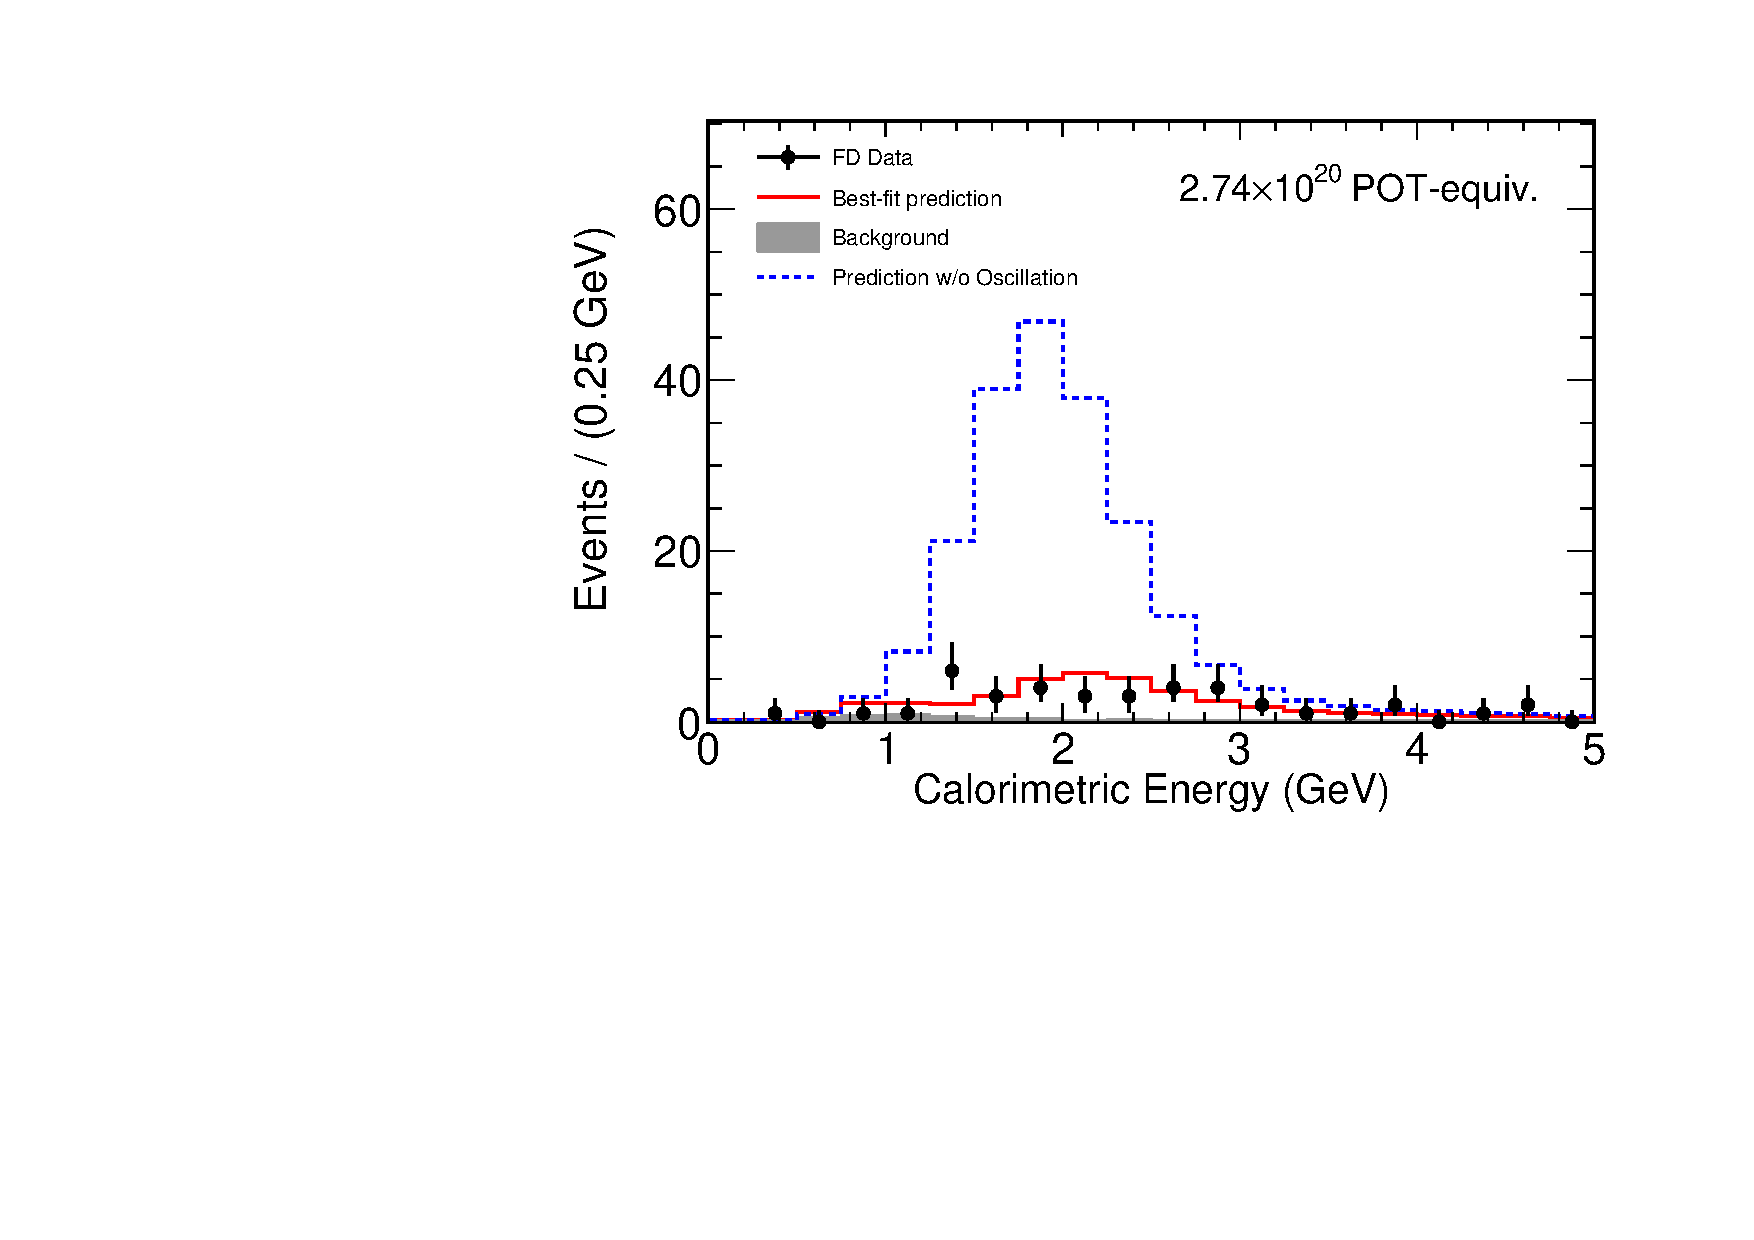
\includegraphics[width=.4\textheight, angle=-90]{figures/results/fd_data_mc_numi_plots/calE_unblind_wUnosc.pdf}};
    \node [dot, right = 1.0cm, right of=energy] (bre){};
    \node [dot, right = 1.0cm, right of=fd] (brf){};
     \node [dot, right = 1.0cm, right of=nd] (brn){};

   % Draw edges
   \path [line] (reco) |- (sel);
    \path [line] (sel) |- (energy);
    \path [lin] (energy) -- (bre);
    \path [lin] (bre) -- (brf);
    \path [line] (brf) |- (fd);
    \path [line] (brn) |- (nd);
    \path [line] (nd) -- (eff);
    \path [line] (eff) -- (extrap);
    \path [line] (extrap) -- (fit);
    \path [line] (fd) -- (fit);


\end{tikzpicture}

}


\begin{frame}

\frametitle{Reconstruction}

\bangon
\item Pattern recognition algorithms produce useful information from raw data
\gap
\item First step is to resolve individual particle interactions
\gap
\item Use DBSCAN for clustering
\gap
\item Each hit pair assigned a neighbor score with time/space distance metric
\begin{equation*}
L = \bigg( \frac{\Delta t - \Delta \vec{r} / c }{T} \bigg)^2 +
     \bigg( \frac{\Delta \vec{r}}{D} \bigg)^2
\end{equation*}
\begin{center}
 ($D$ and $T$ are configurable, $c$ is speed of light)
\end{center}
\bangoff

\begin{columns}[c]
\column{0.3\textwidth}

\centering

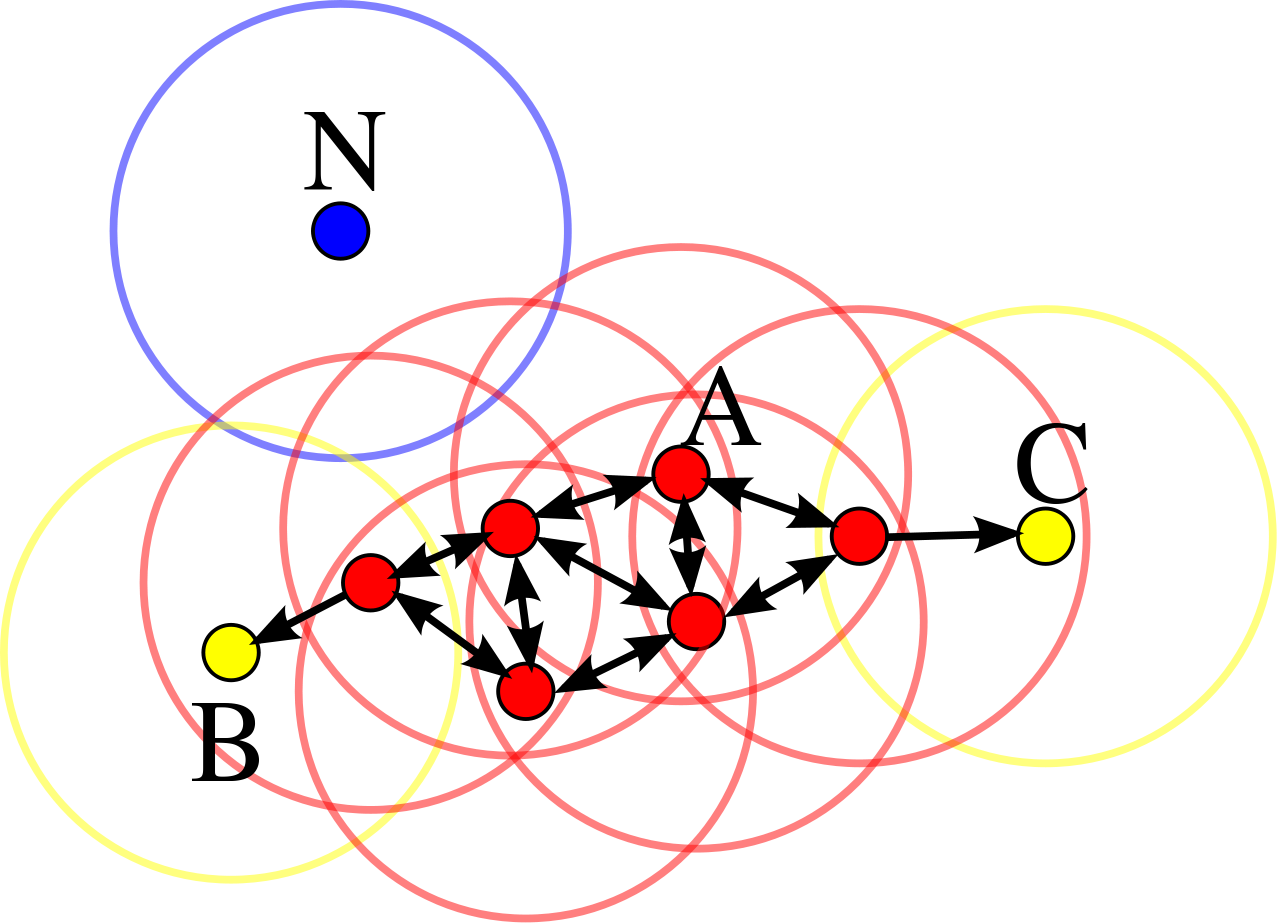
\includegraphics[width=\textwidth]{figures/figures/dbscan.png}

\column{0.7\textwidth}
\bangon
\gap
\item Pairs with score below threshold start a cluster
\gap
\item Cluster boundaries formed in low density regions

\bangoff

\end{columns}

\end{frame}

\frame
{
  \frametitle{Before Clustering}

 \begin{figure} 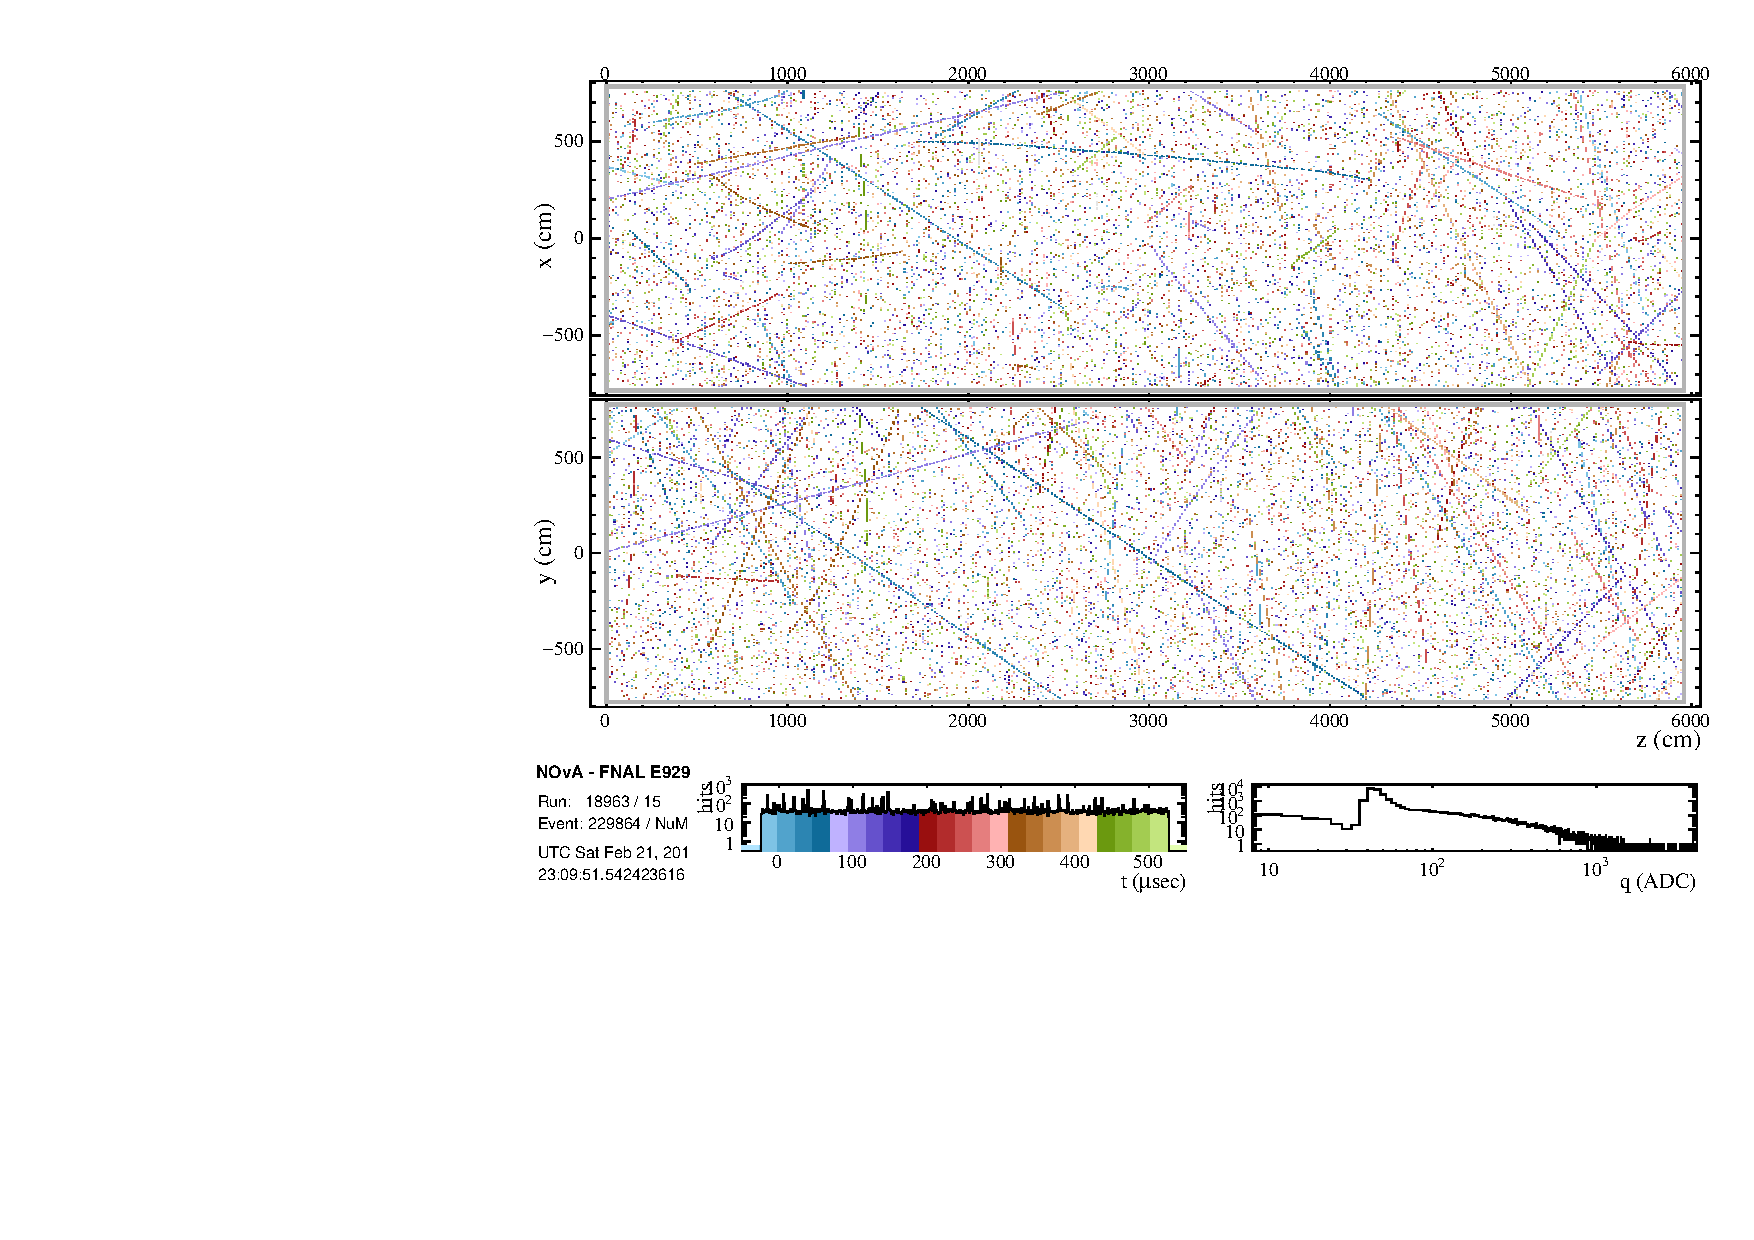
\includegraphics[height=0.9\textwidth, angle=-90]{figures/evd_steps/evd_hits.pdf} \end{figure}
}

\frame
{
  \frametitle{After Clustering}

 \begin{figure} 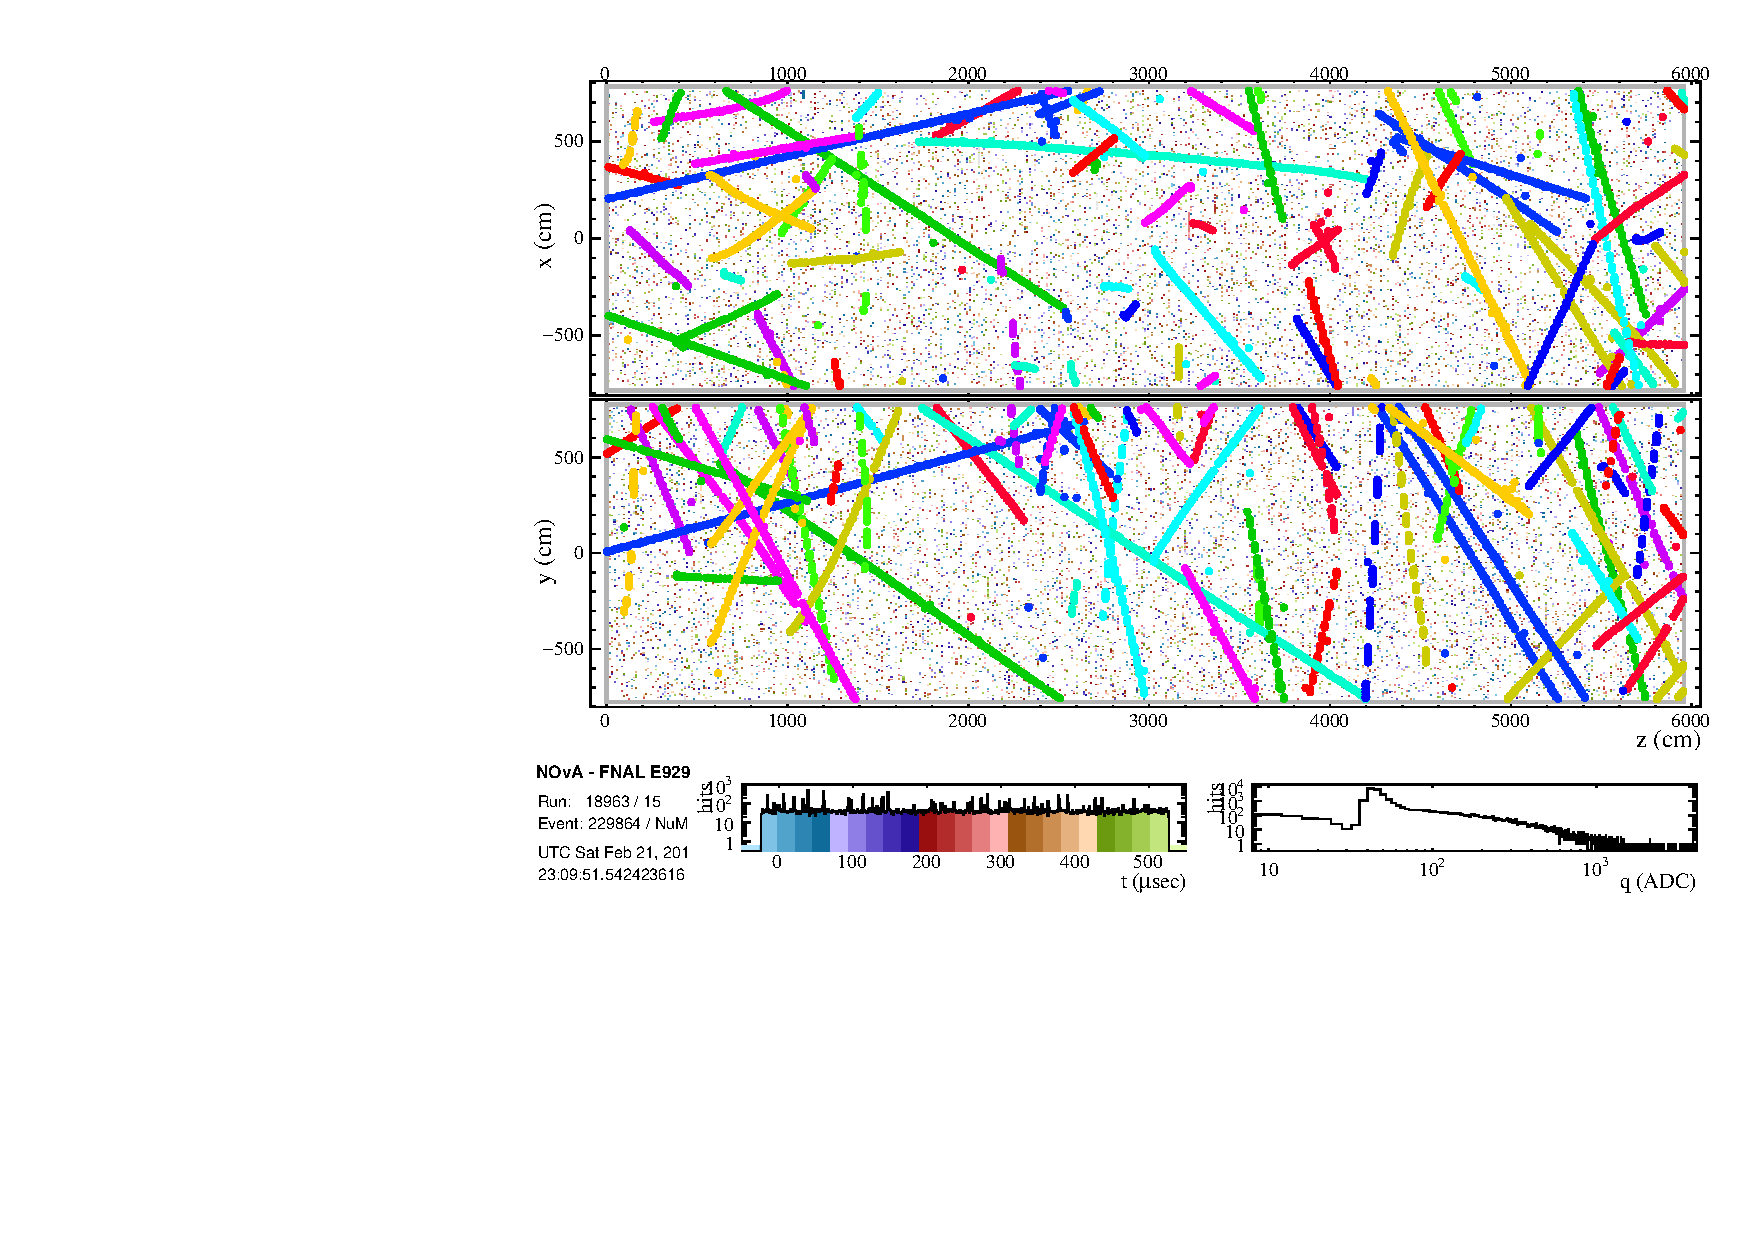
\includegraphics[height=0.9\textwidth, angle=-90]{figures/evd_steps/evd_slice.pdf} \end{figure}
}

\begin{frame}

\frametitle{Further Reconstruction}

\begin{columns}[c]
\column{0.5\textwidth}
  \bangon
  \item Many reconstruction steps can be chained
    \bangon
    \item Hough transform
    \item Kalman filtering
    \item Elastic vertex finding
    \item K-means clustering
    \bangoff
  \gap
  \item Reconstructed features passed to multivariate classifiers
    \bangon
    \item Length
    \item Direction
    \item Gaps
    \item Energy deposition characteristics
    \bangoff
  \gap
  \item Low rate failures compound across multiple steps
  \gap
  \item Tuning for pathological failures can become tedious

  \bangoff
\column{0.5\textwidth}

\centering

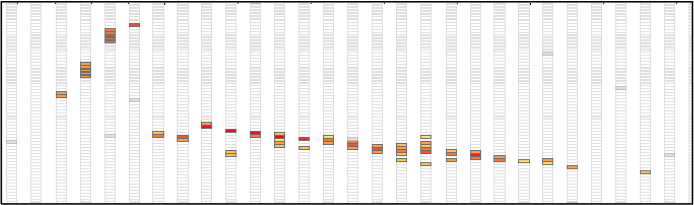
\includegraphics[width=\textwidth]{figures/evd_steps/slice.png}

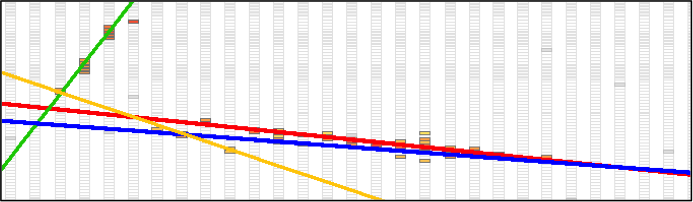
\includegraphics[width=\textwidth]{figures/evd_steps/hough.png}

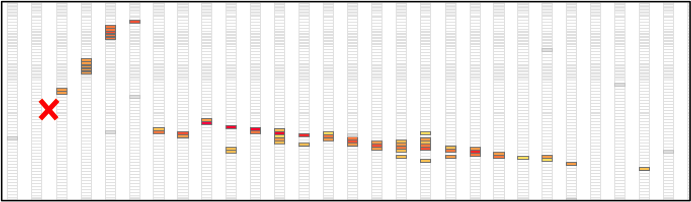
\includegraphics[width=\textwidth]{figures/evd_steps/vertex.png}

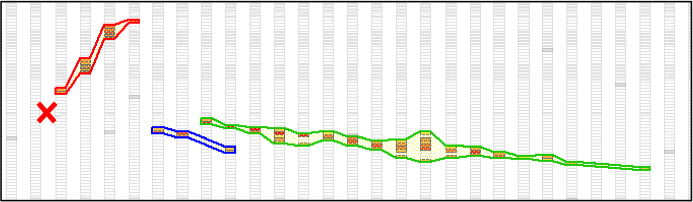
\includegraphics[width=\textwidth]{figures/evd_steps/prongs.png}

\end{columns}


\end{frame}

\begin{frame}
\frametitle{Image Classification}
  \bangon
  \item Classification with raw detector output is potentially less error prone
  \bangon
  \item Just use coarse clusters from DBSCAN
  \item Cut out the rest of the reconstruction
  \bangoff
  \gap
  \item Use methods from computer vision community
  \bangon
  \item Detector output is essentially top and side view image
  \bangoff
  \bangoff
\end{frame}

\begin{frame}
\frametitle{Neural Networks}
  \bangon
  \bang Artificial neural networks (ANN) do well for classification of small images
    \bangon
    \item Each pixel used as input to neural network
    \item Historically successful for optical character recognition (OCR)
    \item[] ... but doesn't scale well above $\sim 100$ pixels
    \bangoff
  \gap
  \item Image processing community finds success in modern ANN variants
    \bangon
    \item Convolutional neural networks (CNN) lead to position invariant feature extraction
    \item New training strategies enable deeper architecture to learn high-level representations
    \item GPU acceleration provides order(s) of magnitude improvement in training time
    \bangoff
  \bangoff

\end{frame}

\begin{frame}
\frametitle{\nova Events as Images}

\begin{columns}[b]
\column{0.5\textwidth}

\bangon
\item Box is drawn around upstream side of slice
\item Box centered on median cell
\bangoff
\vspace{30pt}
\centering
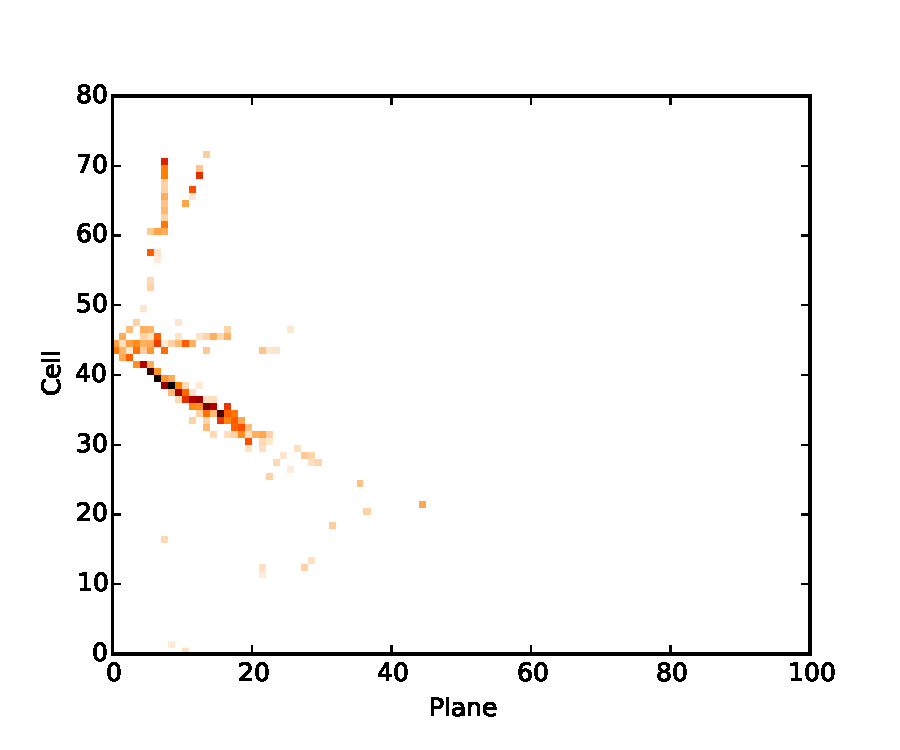
\includegraphics[width=0.85\textwidth]{figures/cnn/view_truetype6_caltype6_event155_y.pdf}


\column{0.5\textwidth}
\centering
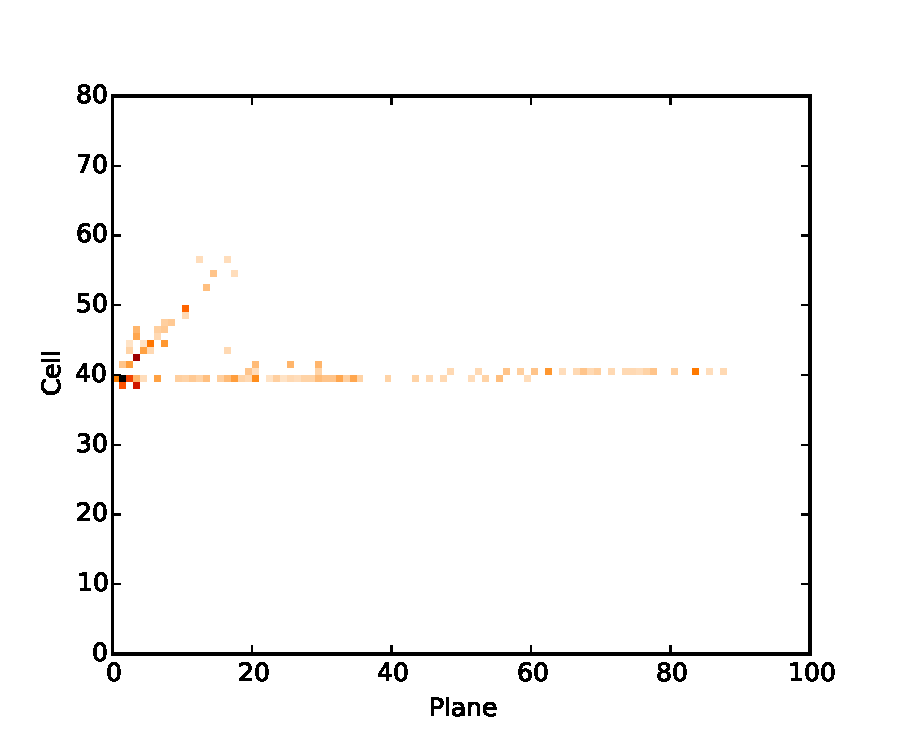
\includegraphics[width=0.85\textwidth]{figures/cnn/view_truetype2_caltype2_event274_x.pdf}

\vspace{-5pt}


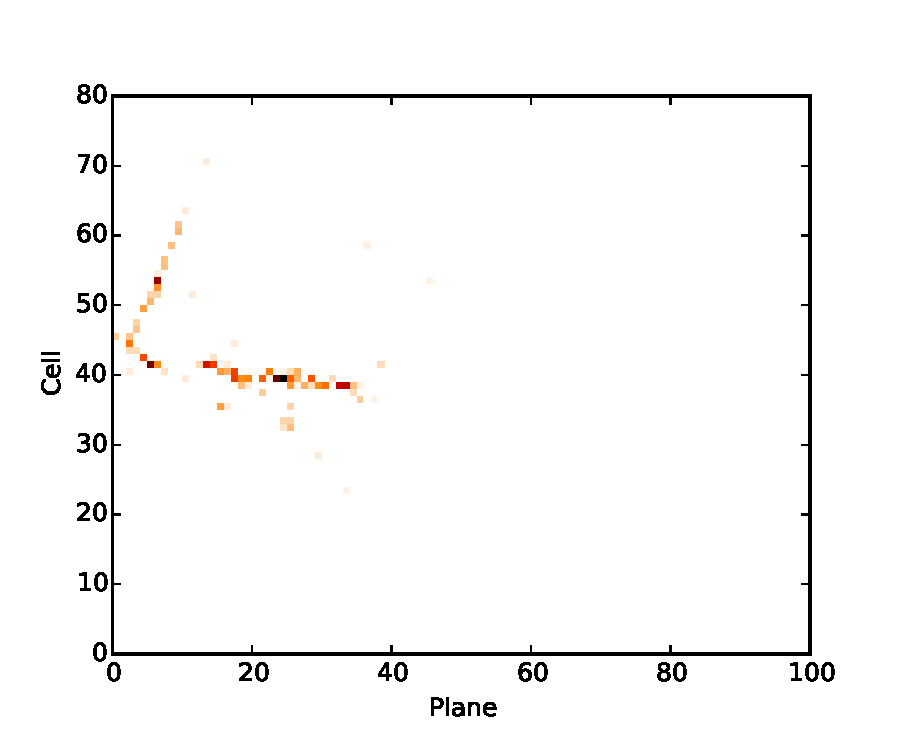
\includegraphics[width=0.85\textwidth]{figures/cnn/view_truetype13_caltype6_event144_x.pdf}

\end{columns}
\end{frame}

\begin{frame}
\frametitle{Neural Networks}

\bangon
\bang A neural network is a ``feedforward graph" of layers, $i$
  \bangon
  \item Each node,  receives input only from previous layers
  \item Nodes take input from each node in previous layer
  \item Each node passes linear combination of inputs, $z$, through a nonlinearity, $g$
  \bong \[ z_{i,j} = \sum_j w_{i,j} a_{i-1, j}; ~~~~~~~~ a_{i,j}  = g(z_{i,j}) \]
  \bangoff
\bangoff
\vspace{-10pt}
\begin{columns}[c]
\column{0.5\textwidth}

  \bangon
  \item[(1)] Input layer: pixels from image
  \item[(2)] Hidden layers: do the classification
  \item[(3)] Output layer: classification result
  \gap
  \item Networks trained using ``backpropagation"
    \bangon
    \item Classification error is minimized in training
    \item Gradient propagated to upstream layers
    \bangoff
  \bangoff
\column{0.5\textwidth}
\centering
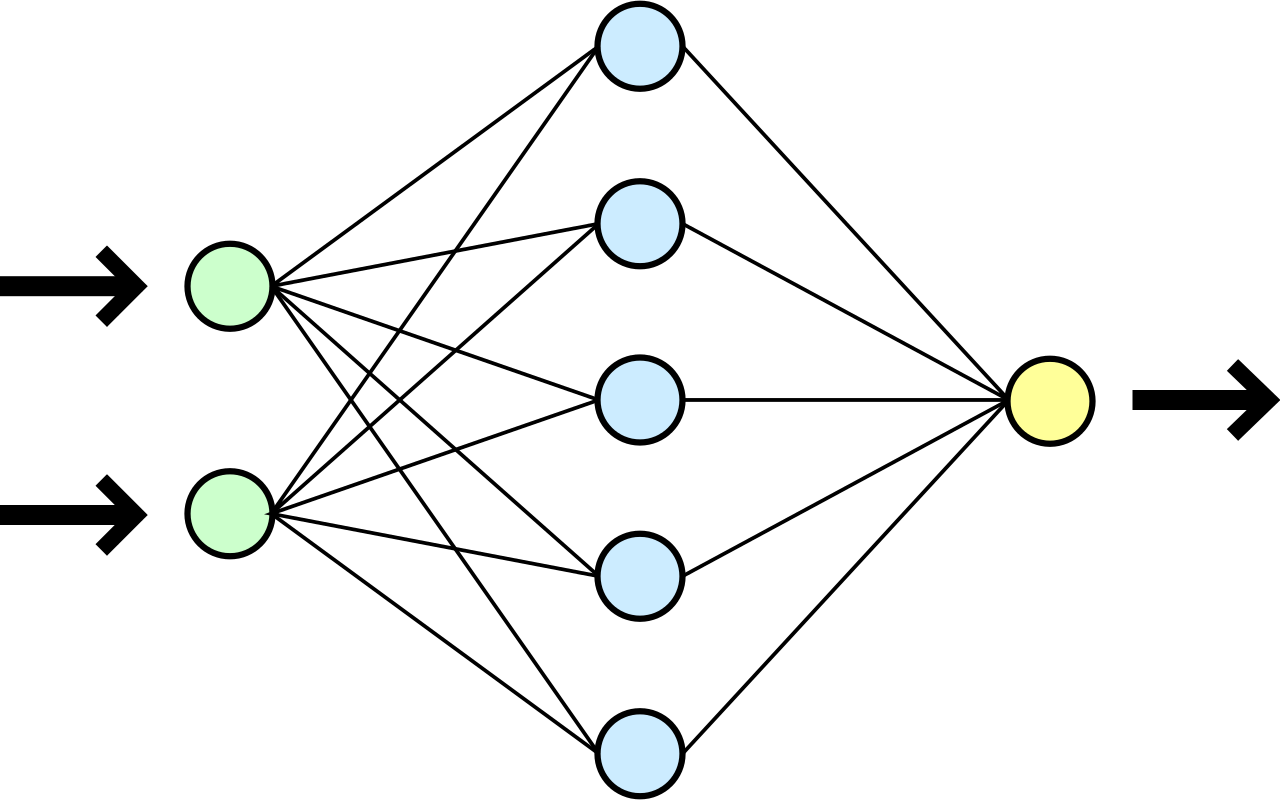
\includegraphics[width=1\textwidth]{figures/figures/basicNN.png}
\end{columns}


\end{frame}


\begin{frame}
\frametitle{Convolutional Layers}


  \bangon
  \item Convolutional layers have demonstrated significant enhancement for image classification
  \bangoff
  \begin{columns}[c]
  \column{0.5\textwidth}
  \centering 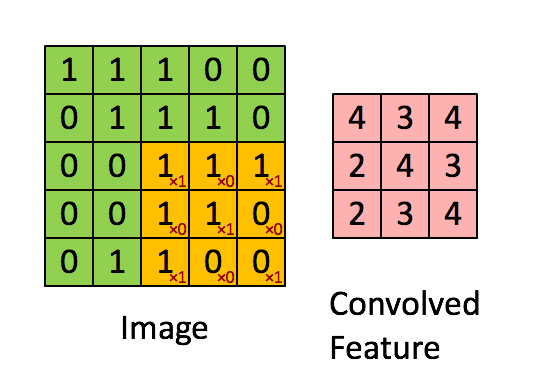
\includegraphics[width=0.7\textwidth]{figures/figures/conv.png}
  \column{0.5\textwidth}
  \centering 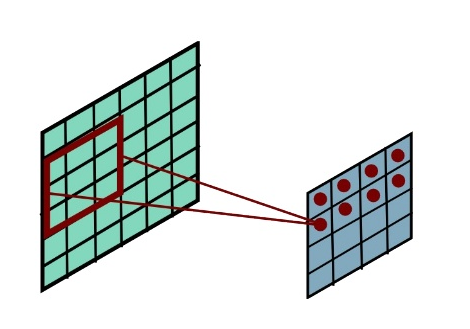
\includegraphics[width=0.7\textwidth]{figures/figures/conv3d.png}
  \end{columns}
  \bangon
  \gap
  \item Convolutional filters are trained to find features in patches of the image
  \gap
  \item Filters are scanned over the input image to produce a feature map
    \bangon
    \item Upshot: position independent feature extraction
    \bangoff
  \gap
  \item Many filters of a particular size are trained in a each convolutional layer
  \gap
  \item Pooling is a common Down-sampling technique
    \bangon
    \item ``Max pooling" simply extracts the maximum pixel (filter output) from each patch
    \bangoff
  \bangoff

\end{frame}

\begin{frame}
\frametitle{GoogLeNet}
\framesubtitle{Network-in-Network, ``Inception"}


  \bangon
  \item Network-in-Network approaches are another recent enhancement
  \item GoogLeNet introduced the ``Inception module"
  \bangoff
  \begin{center}
 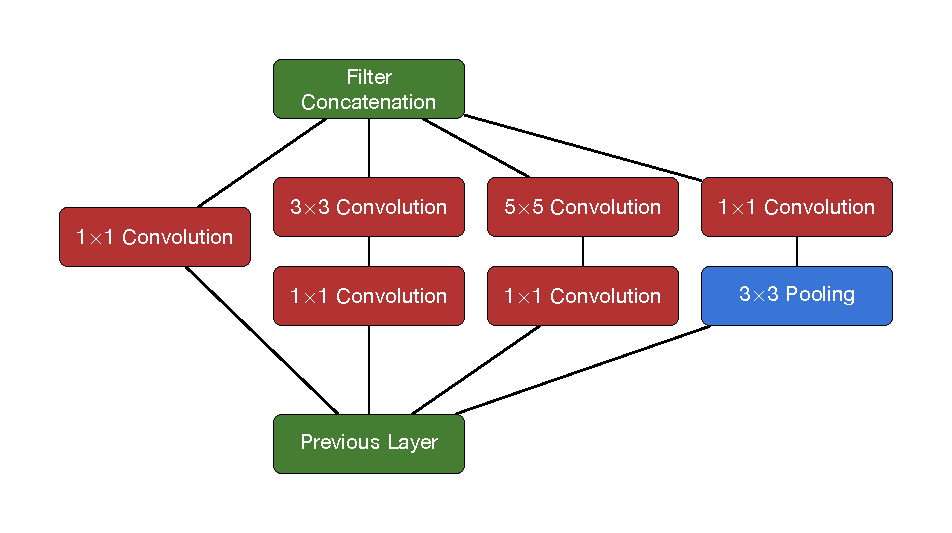
\includegraphics[width=0.5\textwidth]{figures/figures/inception/inception.pdf}
 \end{center}
   \bangon
  \gap
  \item Convolutional layers are arranged side-by-side rather one after another
  \item Sub-layers are concatenated and passed to downstream layers
  \item Downstream layers simultaneously learn structure at different scales
  \item $1\times1$ convolutions are just constant scale factors
    \bangon
    \item Output filters are linear combinations of input filters
    \item Tool for dimensionality reduction
    \bangoff
  \bangoff

\end{frame}



\begin{frame}

\frametitle{Architecture}

  \begin{columns}
  \column{0.28\textwidth}
   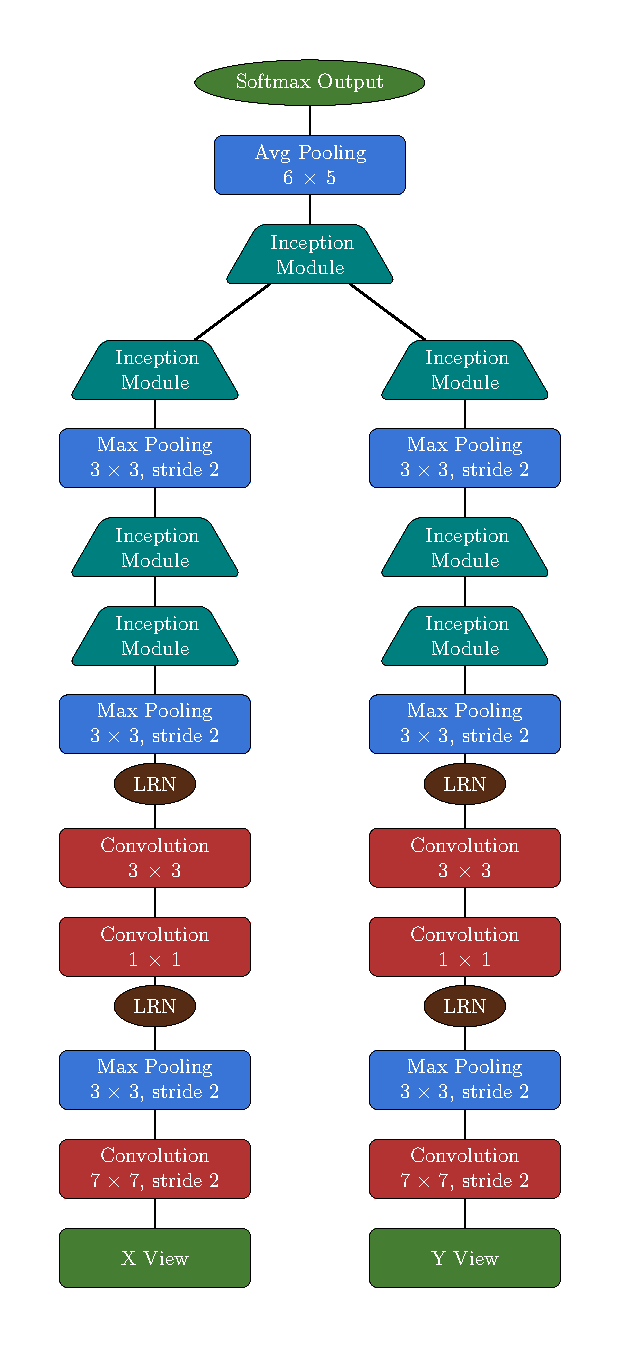
\includegraphics[height=0.9\textheight]{figures/arch/arch.pdf}
  \column{0.72\textwidth}
  \begin{itemize}
  \item Inspired by GoogLeNet, but much more compact
  \bangon
  \bong Szegedy, Christian, et al. ``Going deeper with convolutions." arXiv preprint arXiv:1409.4842 (2014).
  \bangoff
  \gap
  \item Repeated convolution, pooling, inception structures
  \gap
  \item Local Response Normalization (LRN) for smoothing
  \gap
  \item Regularization to prevent overtraining
    \bangon
    \item Jitter tweaks pixel/hit intensity
    \item Dropout cuts out information during training
    \bangoff
  \end{itemize}
  \end{columns}
\end{frame}






\begin{frame}
\frametitle{Classifier Output}
  \begin{center}
   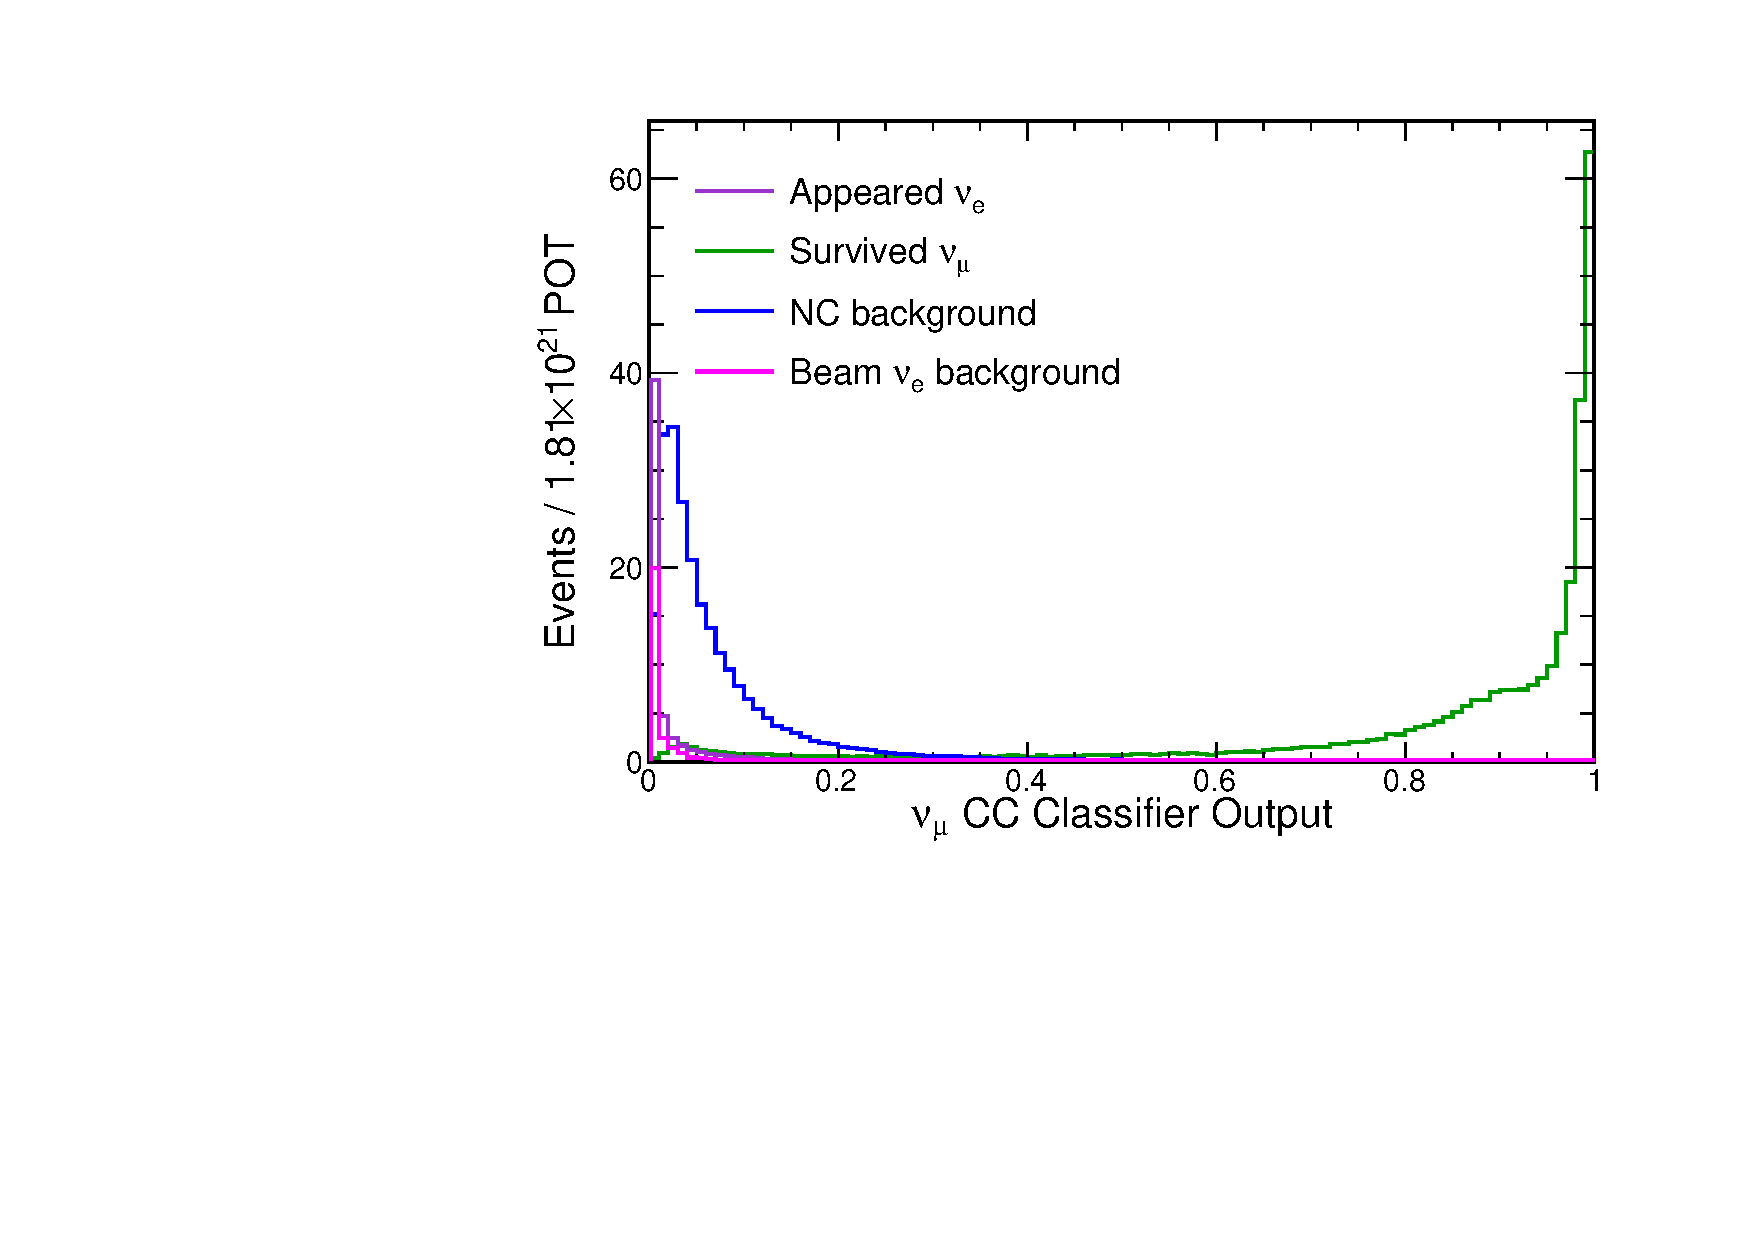
\includegraphics[height=0.7\textwidth, angle=-90]{figures/cnn/numu_pid_dist.pdf}
  \end{center}

  \bangon
  \item Classifier output shows nice separation for beam backgrounds
  \bangoff
\end{frame}


\begin{frame}

\frametitle{Selection Comparison}
  \begin{center}
   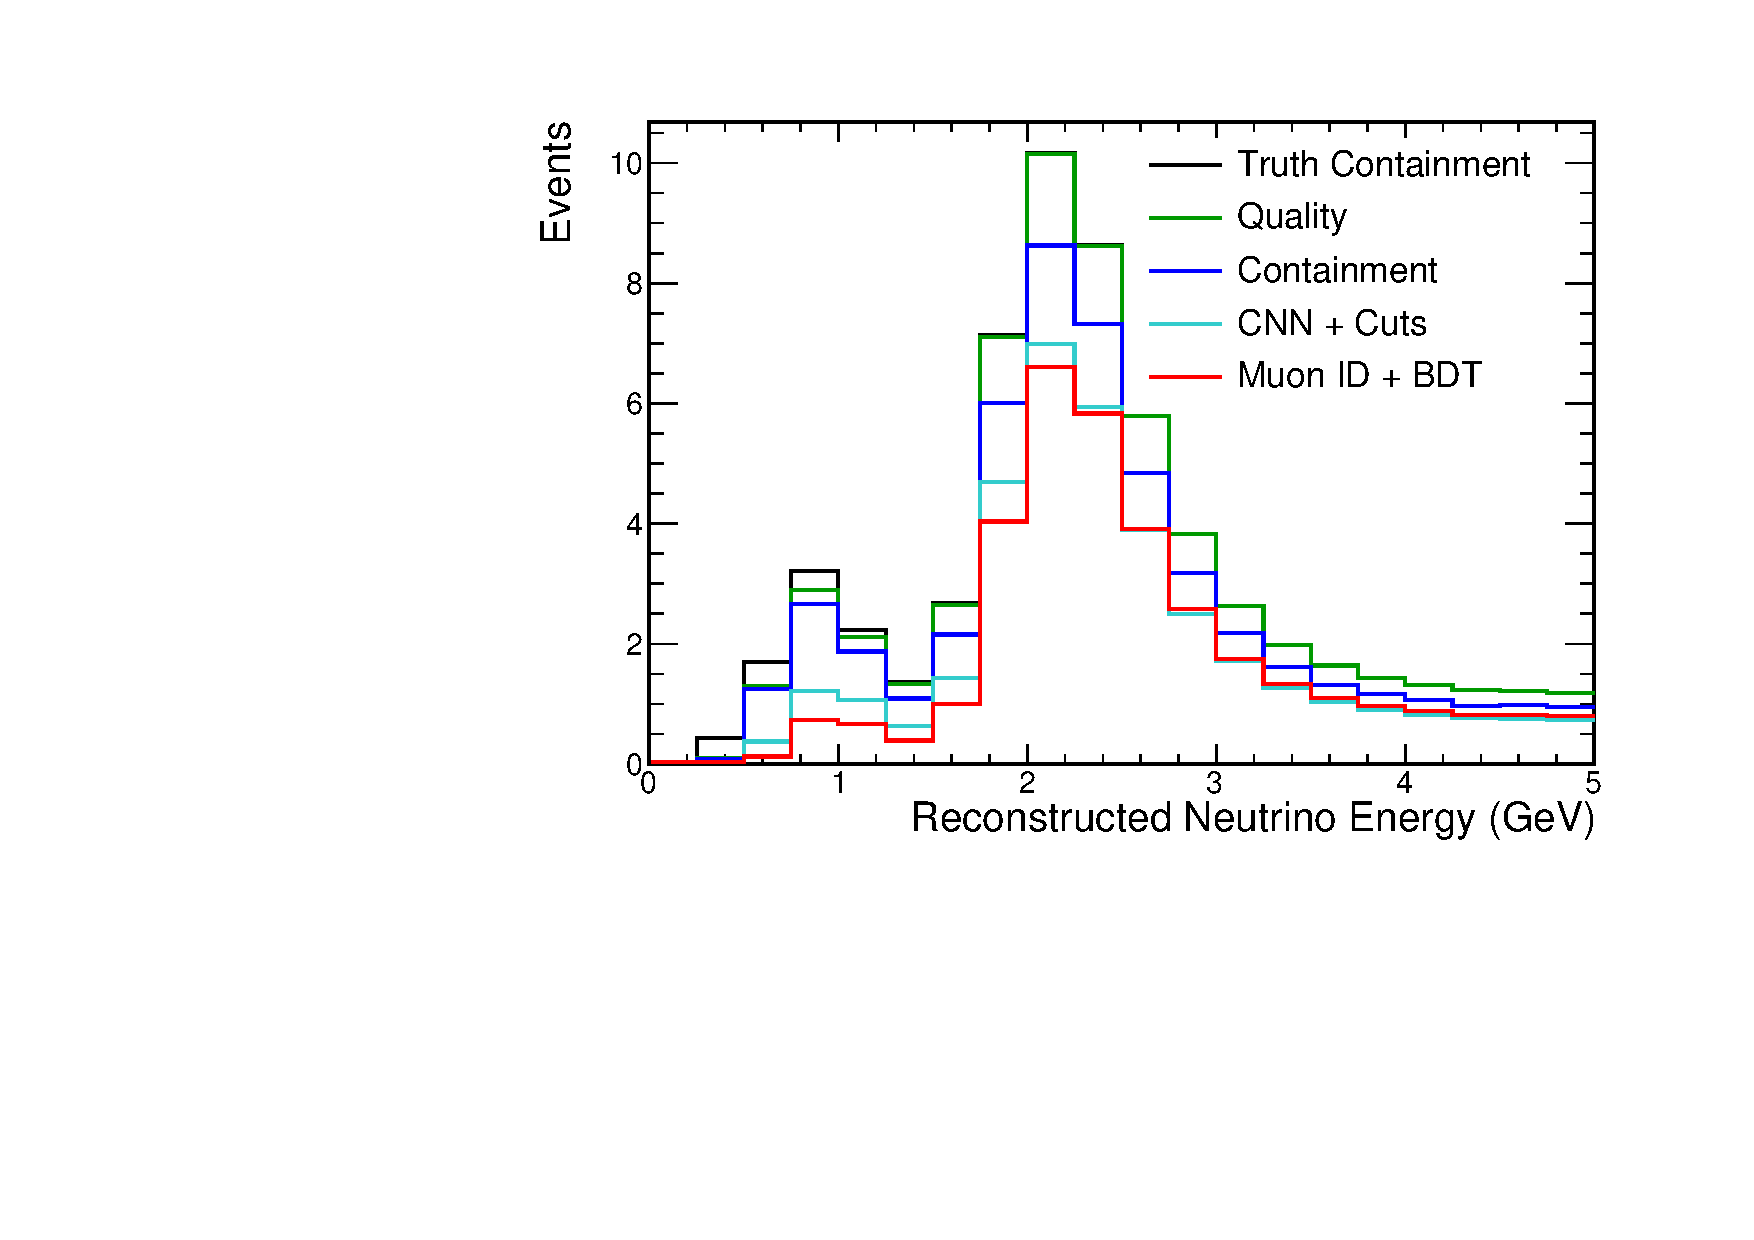
\includegraphics[height=0.7\textwidth, angle=-90]{figures/selection/cosmic_sig_osc.pdf}
  \end{center}
  \gap
  \bangon
  \item Convolutional Neural Network is more efficient, especially at low energies
  \bangoff
\end{frame}


\begin{frame}
\frametitle{Summary}
\bangon
\item \nova studies neutrino oscillations with a beam and two detectors
\gap
\item Reconstruction involves machine learning and pattern recognition algorithms
\gap
\item Treating data as images with a convolutional neural network has been successful
\bangoff
\end{frame}



\end{document}
